\documentclass[12pt,pdftex,noinfoline]{imsart}

\RequirePackage[OT1]{fontenc}
\usepackage{amsthm,amsbsy,amsmath,amsfonts,natbib,mathtools,amssymb}
\usepackage{mathrsfs}
\RequirePackage{hypernat}
\usepackage[ruled, vlined, lined, commentsnumbered]{algorithm2e}
%\usepackage[ruled,section]{algorithm}
%\usepackage{algorithmic}
\usepackage{graphicx}
\usepackage{verbatim}
\usepackage{times}
\usepackage{hyperref}
\usepackage[usenames,dvipsnames,svgnames,table]{xcolor}
\hypersetup{citecolor=MidnightBlue}
\hypersetup{linkcolor=MidnightBlue}
\hypersetup{urlcolor=MidnightBlue}
\usepackage{enumerate}
\usepackage{fullpage}
\usepackage[margin=1in,footskip=.40in]{geometry}
\usepackage{dsfont}
\usepackage{wrapfig}


\usepackage{amsmath, amssymb}
\usepackage{cleveref}
\usepackage{algorithm2e}
\crefname{algocf}{alg.}{algs.}
\Crefname{algocf}{Algorithm}{Algorithms}
\RestyleAlgo{ruled}

\makeatletter
\newcommand*\bigcdot{\mathpalette\bigcdot@{.5}}
\newcommand*\bigcdot@[2]{\mathbin{\vcenter{\hbox{\scalebox{#2}{$\m@th#1\bullet$}}}}}
\makeatother

\renewcommand{\d}{\mathrm{d}}
\newcommand{\E}{\operatorname{\mathbb E}}

\newcommand\numberthis{\addtocounter{equation}{1}\tag{\theequation}}

%\DeclareMathOperator*{\argmin}{\arg\min}
%\DeclareMathOperator*{\argmax}{\arg\max}

\numberwithin{equation}{section}
\newtheorem{thm}{Theorem}[section]
\newtheorem{lemma}{Lemma}[section]
\newtheorem{corollary}{Corollary}[section]
\newtheorem{prop}{Proposition}[section]
\theoremstyle{remark}
\newtheorem{example}{Example}[section]
\newtheorem{remark}{Remark}[section]

\newtheorem*{thm1}{Claim A}
\newtheorem*{thm2}{Claim B}
\newtheorem*{thm3}{Claim C}
\newtheorem*{thm4}{Claim D}
\def\conditionA{Condition $A$}
\def\conditionAp{Condition $\tilde A$}
\def\conditionB{Condition $B$}
\newtheorem*{con0}{\conditionA}
\newtheorem*{con1}{\conditionAp}
\newtheorem*{con2}{\conditionB}

\def\given{\,|\,}
\def\P{\mathbb{P}}
\def\E{\mathbb{E}}
\def\reals{\mathbb{R}}
%\def\argmin{\mathop{\text{arg\,min}}}
\def\ones{\mathds{1}}
\def\indicator{}
\let\hat\widehat
\let\what\widehat
\let\tilde\widetilde
\def\Var{\textsf{Var}}

\newcommand{\argmin}{\mathop{\rm argmin}}
\newcommand{\ess}{\mathop{\rm ess}}
\newcommand{\argmax}{\mathop{\rm argmax}}
\newcommand{\lnorm}[2]{\|{#1} \|_{{#2}}}
\newcommand{\indc}[1]{{\mathbf{1}_{\left\{{#1}\right\}}}}
%\newcommand{\norm}[1]{\|{#1} \|}
\newcommand{\norm}[1]{\left\|{#1} \right\|}
\newcommand{\hf}{{1/2}}
\newcommand{\wh}{\widehat}
\newcommand{\wt}{\widetilde}
\newcommand{\Norm}[1]{\|{#1} \|}
\newcommand{\Fnorm}[1]{\lnorm{#1}{\rm F}}
\newcommand{\fnorm}[1]{\|#1\|_{\rm F}}
\newcommand{\opnorm}[1]{\|#1\|_{\rm op}}
\newcommand{\nnorm}[1]{\|#1\|_{\rm *}}
\newcommand{\Prob}{\mathbb{P}}
\newcommand{\Expect}{\mathbb{E}}
\newcommand{\Span}{{\rm span}}
\newcommand{\rank}{\mathop{\sf rank}}
\newcommand{\sgn}{\mathop{\rm sign}}
\newcommand{\rt}{\mathop{\sf root}}
\newcommand{\R}{\mathop{\sf R}}
\newcommand{\Tr}{\mathop{\sf Tr}}
\newcommand{\diag}{\mathop{\text{diag}}}
\newcommand{\supp}{{\rm supp}}
\newcommand{\iprod}[2]{\left \langle #1, #2 \right\rangle}
\newcommand{\pth}[1]{\left( #1 \right)}
\newcommand{\qth}[1]{\left[ #1 \right]}
\newcommand{\sth}[1]{\left\{ #1 \right\}}
\newcommand{\calL}{\mathcal{L}}
\newcommand{\floor}[1]{{\left\lfloor {#1} \right \rfloor}}
\newcommand{\TV}{{\sf TV}}
\newcommand{\blue}{\color{blue}}
\newcommand{\nb}[1]{\texttt{\blue[#1]}}

\def\bra#1{\langle #1 \vert}
\def\ket#1{\vert #1 \rangle}
\def\braket#1#2{\langle #1 \vert #2 \rangle}
%\def\bind#1#2{\ket{#1}\bra{#2}}
\def\bind#1#2{\ket{#1}|\ket{#2}}
\def\bind#1#2{#1 \| #2}
\let\tilde\widetilde
\def\softmax#1{\mbox{Softmax}\left(#1\right)}
\def\emph#1{\vskip5pt\noindent{\it\bfseries #1}}
\def\task#1{\vskip5pt\noindent{\it\bfseries #1.}}
\def\qkv#1#2#3{\mbox{CrossAttention}(Q\!\leftarrow\!#1,\; K\!\leftarrow\!#2,\; V\!\leftarrow\!#3)}
\def\crossattend#1#2#3#4{\mbox{CrossAttention}_{#4}(Q\!\leftarrow\!#1,\; K\!\leftarrow\!#2,\; V\!\leftarrow\!#3)}

\renewcommand{\baselinestretch}{1.05}

\usepackage{cleveref}
\crefname{algocf}{alg.}{algs.}
\Crefname{algocf}{Algorithm}{Algorithms}

\newcommand{\MLP}{\text{MLP}}
\newcommand{\FeedForward}{\text{FeedForward}}
\newcommand{\Softmax}{\text{Softmax}}


\begin{document}

\setlength{\parskip}{0.5em}
\begin{frontmatter}
%{\bf\Large Relational Abstracters and Symbolic Message Passing: \\[7pt] Transformer Modules for Relational Reasoning}
%\vskip10pt
{\bf\Large Abstractors: Transformer Modules for \\[7pt] Symbolic Message Passing and Relational Reasoning}
%\affil[**]{Department of Statistics and Data Science, Yale University}
\begin{aug}
\vskip15pt
\address{
\begin{tabular}{ccccc}
{\normalsize\rm\bfseries Awni Altabaa} & {\normalsize\rm\bfseries Taylor Webb} & {\normalsize\rm\bfseries Jonathan  Cohen} & {\normalsize\rm\bfseries John Lafferty}\\[5pt]
\end{tabular}
\\[10pt]
\today
\vskip10pt
}
\end{aug}
\begin{abstract}
    Abstracter, Abstractest
\end{abstract}
\end{frontmatter}

%\begin{enumerate}
    \item Introduction
    \item Encoding relations as abstract values
    \item Relational abstractors as transformer modules
    \item Function classes 
    \item External memory 
    \item Experiments
    \item Discussion
\end{enumerate}

\section{Introduction}
\label{sec:intro}

Relational learning refers to the inference of rules that operate in terms of pairwise relationships between 
objects, independent of how the objects may be represented. Common relations are ``less than'' applied to natural numbers, ``same color as'' applied to visual objects, and ``friend of'' applied to social relationships. Consider the task of sorting objects. A standard 52-card deck of playing cards has 13 ranks in each of four suits: clubs, diamonds, hearts, and spades. The cards might be sorted using the relation that takes 
the suit as the primary attribute, and the rank as the secondary attribute; this would be the typical 
way of ordering cards in many games. If a sorting algorithm is learned that depends 
only on the relations between objects, it can in principle be applied in a new domain with little 
or no modification. 

Reasoning in terms of relations and analogies is a hallmark of human intelligence. 
Indeed, the Wisconsin card sorting task \citep{berg} has been used for decades as an indicator of decision making function in prefrontal cortex \citep{monchi}. Recognizing the importance of this type of learning, which is largely separate from function approximation for sensory tasks such as image and audio processing, machine learning research has explored several novel frameworks for relational learning \citep{TEM, NTM,episodicControl,esbn,mondal23learned,musslick2021rationalizing,battaglia,barrett:2018,santoro1} .

In this paper we propose a framework that casts relational learning in terms of transformers. 
The success of transformers lies in combining the function approximation capabilities of deep learning with the use of attentional mechanisms to support richly context-sensitive processing \citep{transformers,vaswani2017attention,kerg2020untangling}. Yet it is clear that transformers are missing core capabilities required for modeling human thought \citep{mahowald2023dissociating}.  In particular, they lack mechanisms required to emulate forms of flexibility and efficiency exhibited by the human brain, including an ability to support analogy and abstraction from limited data. The algorithmic challenge is to provide ways of binding domain-specific information to low dimensional, abstract representations that can be used to compute a given function in any setting for which it is relevant. 

Our approach is motivated by a type of inductive bias for relational learning architectures we call the ``relational bottleneck," which is motivated by principles of cognitive neuroscience that shed light on the brain subsystems involved when natural intelligence shows an ability to flexibly generalize abstract structure across domains of processing. In particular, the framework of complementary learning systems \citep{McClelland:1995, Kumaran:2016} describes two distinct types of neural mechanisms for learning and memory around which the brain is organized, implementing a tradeoff between slow, incremental forms of learning required to encode stable statistical structure present in the environment (semantic memory), and the ability to rapidly encode and remember novel associations and form analogies (episodic memory). In its most basic and simplified form, the ``relational bottleneck'' imposes an inductive bias that constrains the flow of information from sensory or motor subsystems to reasoning and decision making subsystems, by restricting this information to relations, as computed through inner products between distributed representations. In this paper we present a framework that casts this inductive bias in terms of 
an extension of transformers, where specific types of attention mechanisms enforce the relational bottleneck, 
and new types of transformer modules use these attention mechanisms to implement a form of abstraction and relational reasoning.

Our approach was developed while thinking about the ESBN framework \citep{esbn}, which can be seen as 
closely related to the neural Turing machine \citep{NTM}. Both frameworks augment traditional controllers such as 
LSTMs with external stores that can be viewed as computational models of episodic memory. However, the ESBN framework enforces a relational bottleneck by dividing the external memory into ``sensory'' and ``abstract'' sides, with lookups on the sensory side carried out using inner products. The key observation we develop in this paper is that by viewing episodic memory query-key lookups in terms of cross attention operations, the relational bottleneck can be 
naturally implemented in an extension of transformers. Our proposed \textit{abstractor} framework extends ESBN to enable more complex, higher order forms of relational learning by combining it with both the attentional mechanisms and hierarchical structure of transformers. This creates a potentially powerful combination of deep learning and relational learning that enables abstraction and generalization from limited data.






%\newcommand{\MLP}{\text{MLP}}
%\newcommand{\FeedForward}{\text{FeedForward}}
%\newcommand{\Softmax}{\text{Softmax}}
%\newcommand{\reals}{\mathbb{R}}
\def\m{m}


\section{Relational symbolic message-passing}
\label{sec:message_passing}

At a high level, the primary function of a relational abstractor is to compute abstract relational features of its
inputs. That is, given a set of input objects $o_1, \ldots, o_\m$, the relational abstractor computes a function on
the set of pairwise relations between objects $\{ R(o_i, o_j) \}_{i,j}$, where $R(\cdot, \cdot)$ is a relation between a pair of objects; the relations are learned to carry out a specific prediction task,
% JDC ADDITION:
in such a form that they can be generalized to any arbitrarily large set of inputs that are appropriate for the task.

At the core of relational abstractors is an operation we refer to as \textit{relational symbolic message-passing}.
The input to this operation is a relation tensor $R = \left[R(o_i, o_j)\right]_{i,j=1}^\m$, where $R(o_i, o_j) \in \mathbb{R}^{d_r}$ is a vector describing the relation between object $o_i$ and object $o_j$. We will come back to how an abstractor computes the relation tensor,
% JDC ?OK:
after considering how the symbols on which it operates can be learned.

The first set of learnable parameters of symbolic message-passing is a set of symbols $s_1, \ldots, s_\m \in \mathbb{R}^{d_s}$, where the hyperparameter $d_s$ is the dimension of the symbolic vectors. We call these parameters \textit{symbols} because each of them references (or ``is bound to") a particular object, but they are independent of the values of these objects. That is, the $i$th symbol references the $i$th object, but the value of $s_i$ is independent of the value of $o_i$. The use of those learned input-indpendent symbols is how symbolic message-passing achieves its abstraction.

In relational symbolic message-passing, we perform message-passing on these learned symbolic parameters according to the relation tensor $R$. In general, this message-passing operation can be described as a set-valued function of the form
\begin{equation}
    \label{eq:symbolic_message_passing}
    s_i \leftarrow \text{Update}\Big( s_i, \ \left\{ \left(R[i,j], s_j\right)\right\}_{j\in[m]}\Big), \quad i = 1, \ldots, m
\end{equation}
That is, the value of the $i$th symbol is updated as a function of the set of tuples $(R[i,j], s_j)$ of the relations with all other objects and the symbols of these objects. The symbols $s_j$ are naturally viewed
as values on the nodes of a graph, and the relations $R[i,j]$ are naturally viewed as weights on the edges. A simple but important special case of this is
\begin{equation}
    \label{eq:linear_symbolic_mp}
    s_i \leftarrow \sum_{j=1}^{m} R[i,j] s_j, \quad i=1, \ldots, m
\end{equation}
In the above, suppose that $d_r = 1$. Otherwise, the above operation is done for each dimension of the relation $R$ and the result is concatenated, as in multi-head attention.

Following message-passing, each updated symbol $s_i$, can be passed through a feedforward neural network $f:\reals^{d_s}\rightarrow \reals^{d_s}$ to compute a non-linear function of the output. %Empirically, a residual connection and layer normalization may be useful, as in a transformer.
This message-passing operation can be repeated multiple times to iteratively update the symbolic vectors.  The output of relational symbolic message-passing is the set of symbols $A$ at the end of this sequence of message-passing operations. The overall procedure is summarized in Algorithm~\ref{alg:relational_abstractor}. In Section~\ref{sec:function_spaces} we characterize the class of functions on relations that this operation can compute.

% JDC: Shouldn't $d_s$ be included in the list of hyperparameters below?
\begin{algorithm}[th!]
    \caption{Relational Abstractor}\label{alg:relational_abstractor}
    \SetKwFor{For}{for}{do}{end}
    \SetKwInOut{Input}{Input}
    \SetKwInOut{Output}{Output}
    \SetKwInOut{LearnableParams}{Learnable parameters{\ }}
    \SetKwInOut{HyperParams}{Hyperparameters}

    \Input{Encoder entities: $E = (o_1, \ldots, o_\m) \in \mathbb{R}^{d_e \times m}$}
    \HyperParams{$L$ (number of layers), $H$ (number of heads), feedforward network structure}
    \LearnableParams{Symbols $S \in \reals^{d_s \times m}$, parameters $\{\theta_l\}$ of attention heads and feedforward models}
    \Output{Abstracted sequence: $A = (a_1, \ldots, a_\m) \in \reals^{d_a \times m}$}
    \vspace{1em}

    $A \gets S$

    \For{$l \gets 1$ \KwTo $L$}{
        $A \gets \text{SelfAttention}_{\theta_l}(A)$\;
        $A \gets \crossattend{E}{E}{A}{\theta_l}$\;
        $A \gets\FeedForward_{\theta_l}(A)$\;
        }
\end{algorithm}

\subsection{Computing the relation tensor with relational cross-attention}

Symbolic message passing is the first of the two main
%ingredients
components
of abstractors. What remains is to describe how the abstractor computes the relation tensor $R$. This is
done through a variant of transformer cross-attention that we refer to as \textit{relational cross-attention}.
To motivate this, we first describe how we can compute relations between pairs of objects through inner products.
The inner product operation is a natural way to capture notions of relations and similarity. In Euclidean space,
inner products capture the geometric alignment between vectors. Similarly, for objects with vector representations,
inner products between these vector representations can capture relations between these objects.

In general, we can formulate inner product relations as the standard Euclidean inner product between a pair of transformed object vectors. That is, 
\begin{equation}
    R(o_i, o_j) = \langle \phi(o_i), \psi(o_j) \rangle
    \label{eq:relation_innerproduct}
\end{equation}
This captures a large class of relation functions. In particular, the theory of reproducing kernel Hilbert spaces implies that any continuous, symmetric function on pairs of objects can be approximated with such functions
\citep{universal}. Multi-dimensional relation functions can be achieved by stacking multiple such inner products.
In the next section we frame this explicitly in terms of transformer operations.

% NOTE / TODO: need to describe what we mean by `relations', `relation functions', `inner product relations', etc. in more detail somewhere?
% maybe in intro at high-level
% JDC: I HAD THE SAME INCLINATION ABOVE (IN RESPONSE "The inner product operation is a natural way to capture...).
% ONE THOUGHT WE HAVE HAD IS THAT THEY CAN ALSO BE USED TO CAPTURE CONTRASTIVE RELATIONSHIPS, SINCE THE
% INNER PRODUCT IS SENSITIVE TO THE NORMS OF THE VECTORS (AS LONG AS NO FORM OF NORMALIZATION IS APPLIED, INCLUDING
% SOFTMAX FOR READOUT) -- SIMON CAN TALK ABOUT THIS ON MONDAY.

% comment this out
% \end{document}

\def\bra#1{\langle #1 \vert}
\def\ket#1{\vert #1 \rangle}
\def\braket#1#2{\langle #1 \vert #2 \rangle}
%\def\bind#1#2{\ket{#1}\bra{#2}}
\def\bind#1#2{\ket{#1}|\ket{#2}}
\def\bind#1#2{#1 \| #2}
\let\tilde\widetilde
\def\softmax#1{\mbox{Softmax}\left(#1\right)}
\def\emph#1{\vskip5pt\noindent{\it\bfseries #1}}
\def\task#1{\vskip5pt\noindent{\it\bfseries #1.}}
\def\qkv#1#2#3{Q\!=\!#1,\; K\!=\!#2,\; V\!=\!#3}

\addtocounter{section}{2}
\section{Relational abstractors as transformer modules}

In the previous section we presented relational learning 
in terms of symbolic message passing operations. In this section, 
we formulate these operations as extensions of transformer architectures
in a way that preserves the separation between sensory processing and 
abstract reasoning motivated by principles of brain organization.

The success of transformers lies in combining the inferential capabilities of deep learning with the use of attentional mechanisms to support richly context-sensitive processing \citep{transformers,vaswani2017attention,kerg2020untangling}. At the same time, it is clear that transformers are missing core capabilities required for modeling human thought (e.g., \cite{mahowald2023dissociating}).  In particular, they lack critical mechanisms required to emulate forms of flexibility and efficiency exhibited by the human brain, including an ability to support abstraction from limited data. The algorithmic challenge is to provide ways of binding domain-specific information to low dimensional, abstract representations that can be used to compute a given function in any setting for which it is relevant. 

The ESBN architecture \citep{esbn} enables learning of simple relations and sequential rules. The abstractor 
framework proposed here extends ESBN to enable more complex, higher order forms of relations by combining it with both the attentional mechanisms and hierarchical structure of transformers. This creates a powerful combination of deep learning and relational learning that enables abstraction and generalization from limited data.

\subsection{Relational learning using transformers}

In the abstractor framework, processing occurs in encoder/decoder modules that handle particular types of information, separated from modules for ``abstract inference.'' The encoders/decoders and the abstractor modules communicate through cross attention mechanisms that couple abstract states (or ``symbols'') with specific information in encoder/decoder modules to which they refer in a given problem instance.  The abstract layers are composable to include a hierarchy of abstract modules in which higher order relations are learned from lower level relations, analogous to how convolutional layers are composed in deep neural networks.

The architecture has three types of states: encoder states $E$, decoder states $D$, and abstract states $A$. The encoder and decoder states are vectors
that represent domain-specific information (e.g., sensory or motor), which are often successfully modeled  
by standard deep learning frameworks, including standard transformers. The abstract states $A$ are vectors 
that are learned and processed using similar mechanisms but, critically, without direct exposure to the $E$ and $D$ states.  In particular, the encoder states are separated from the abstract states by a ``relational bottleneck'' 
that only allows information about relations (that is, inner-products) between encoder 
states to influence the transformation of abstract states.

\begin{figure}[t]
    \vspace{-3mm}
    \begin{center}
    \begin{tabular}{cc}
        \hskip-2pt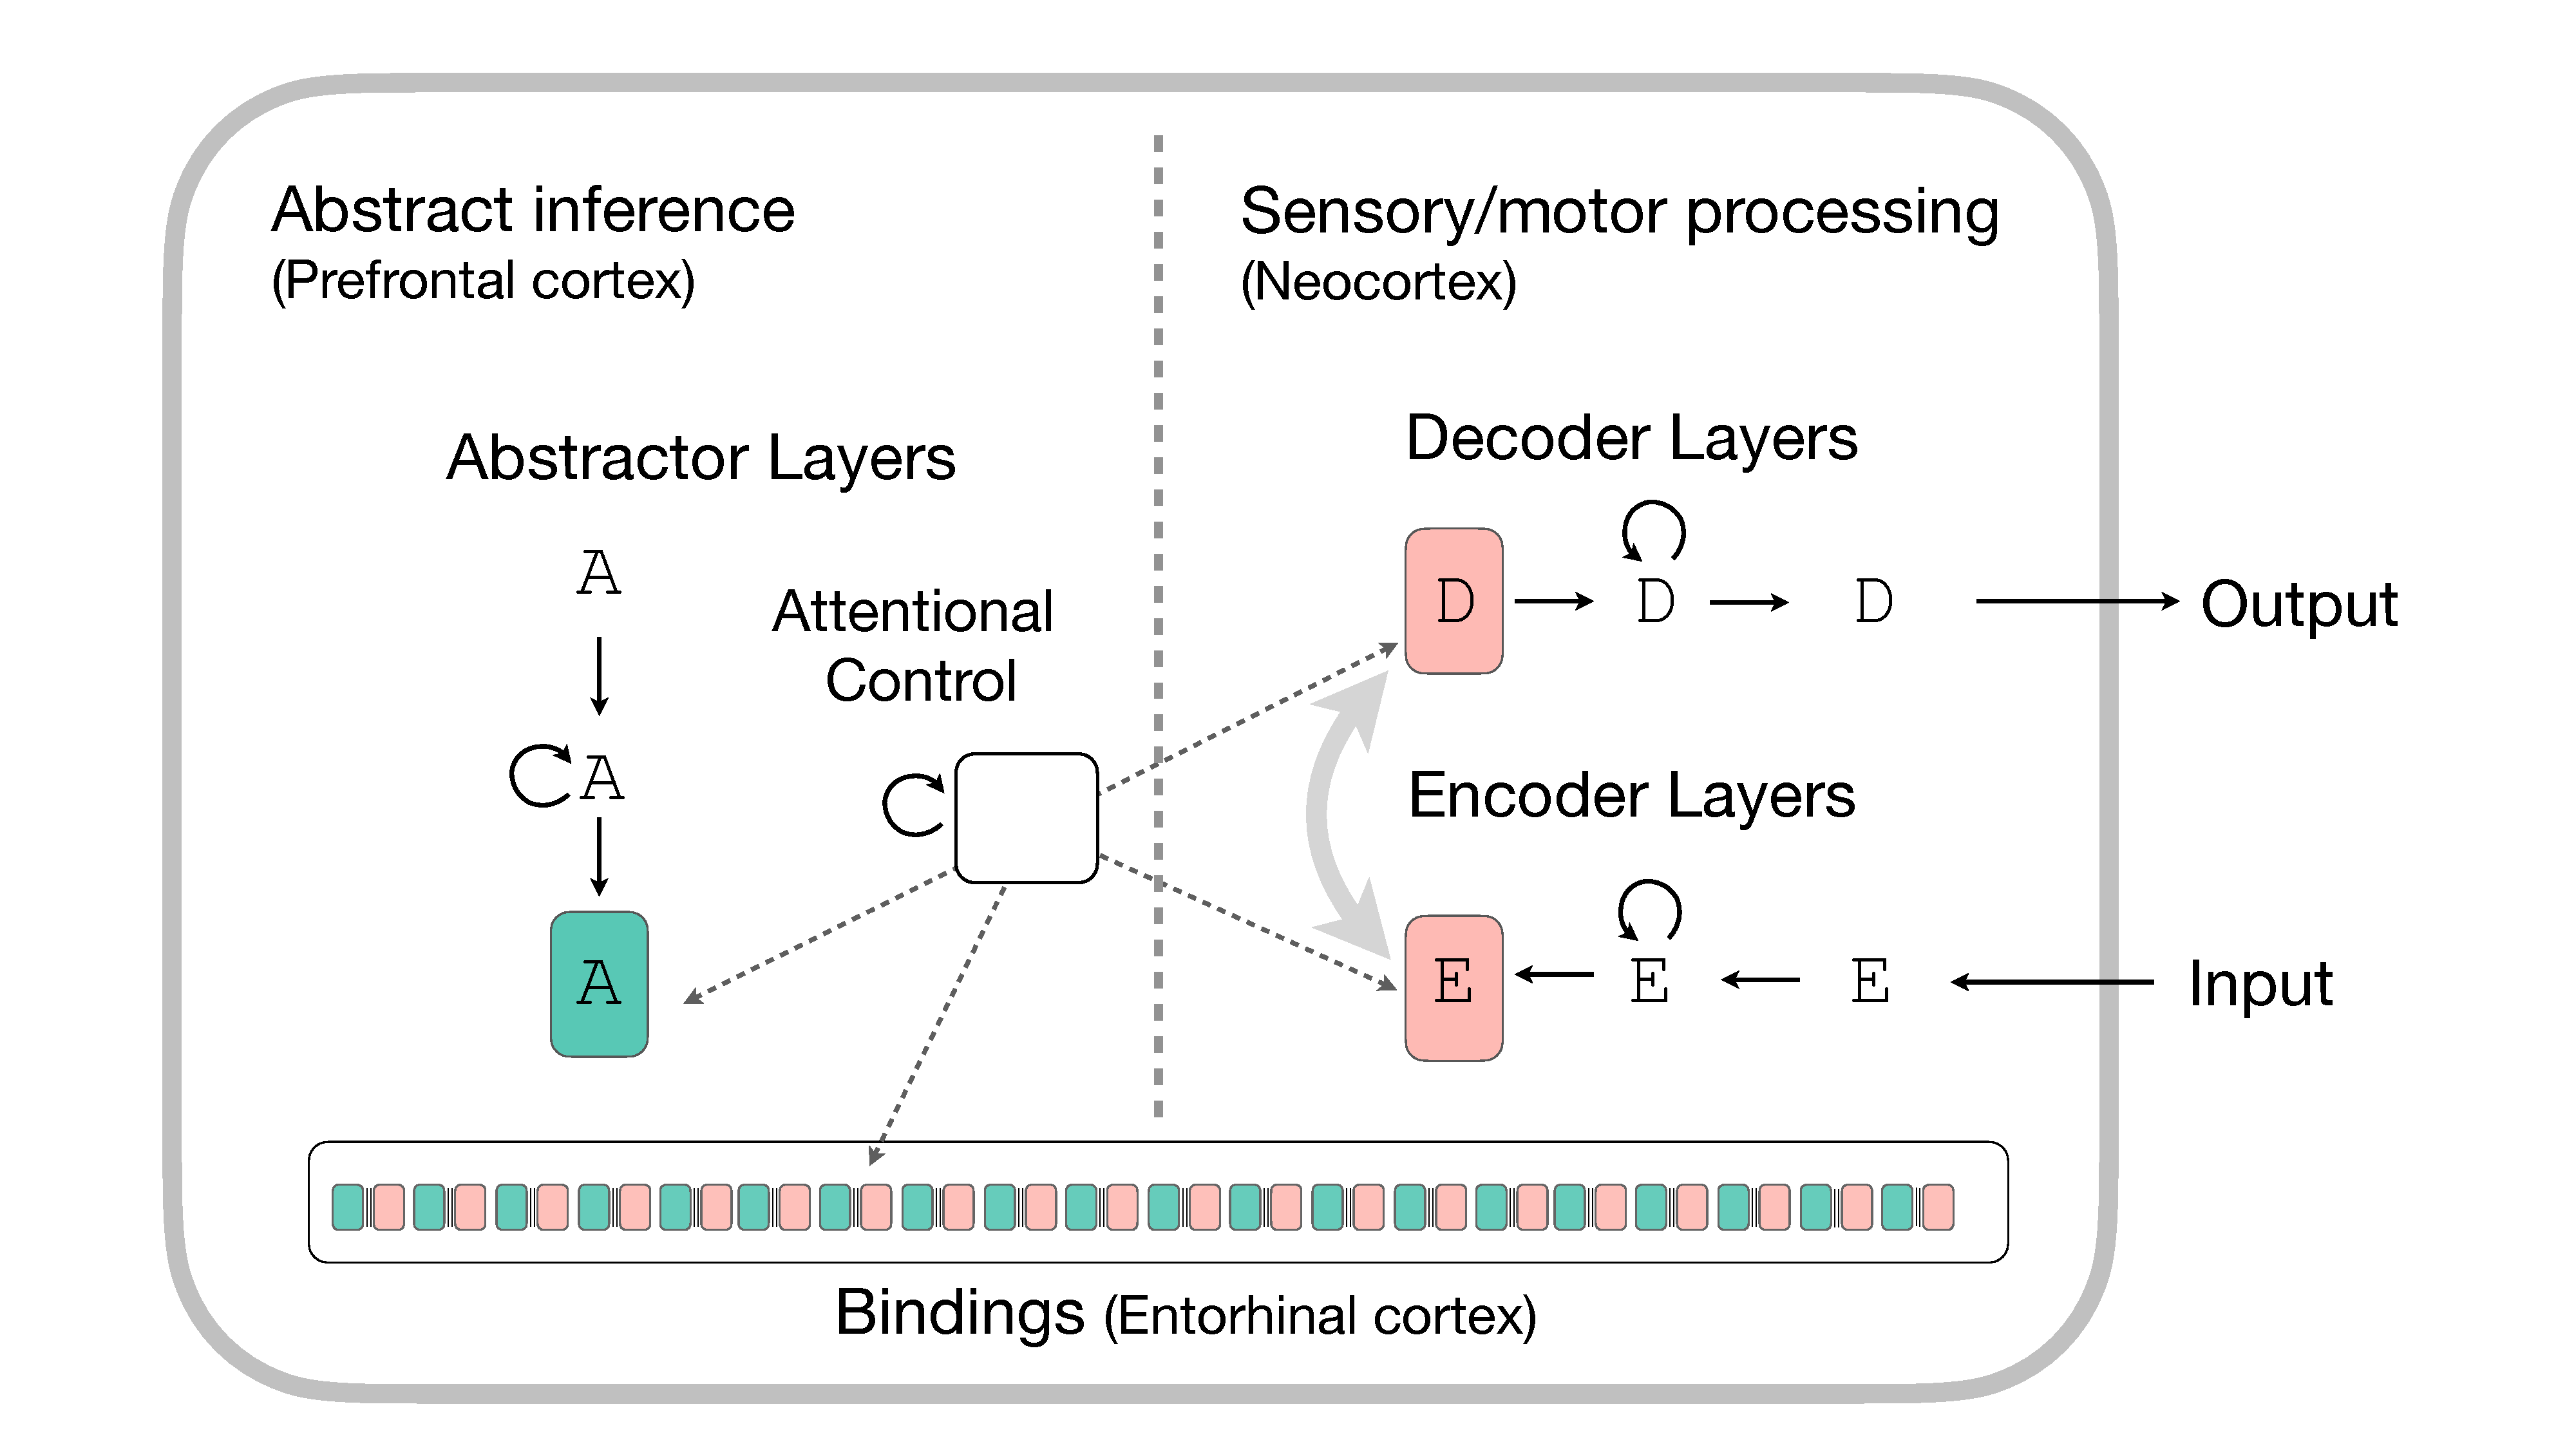
\includegraphics[width=.50\textwidth]{figures/algorithm-diagram2} &
        \hskip-10pt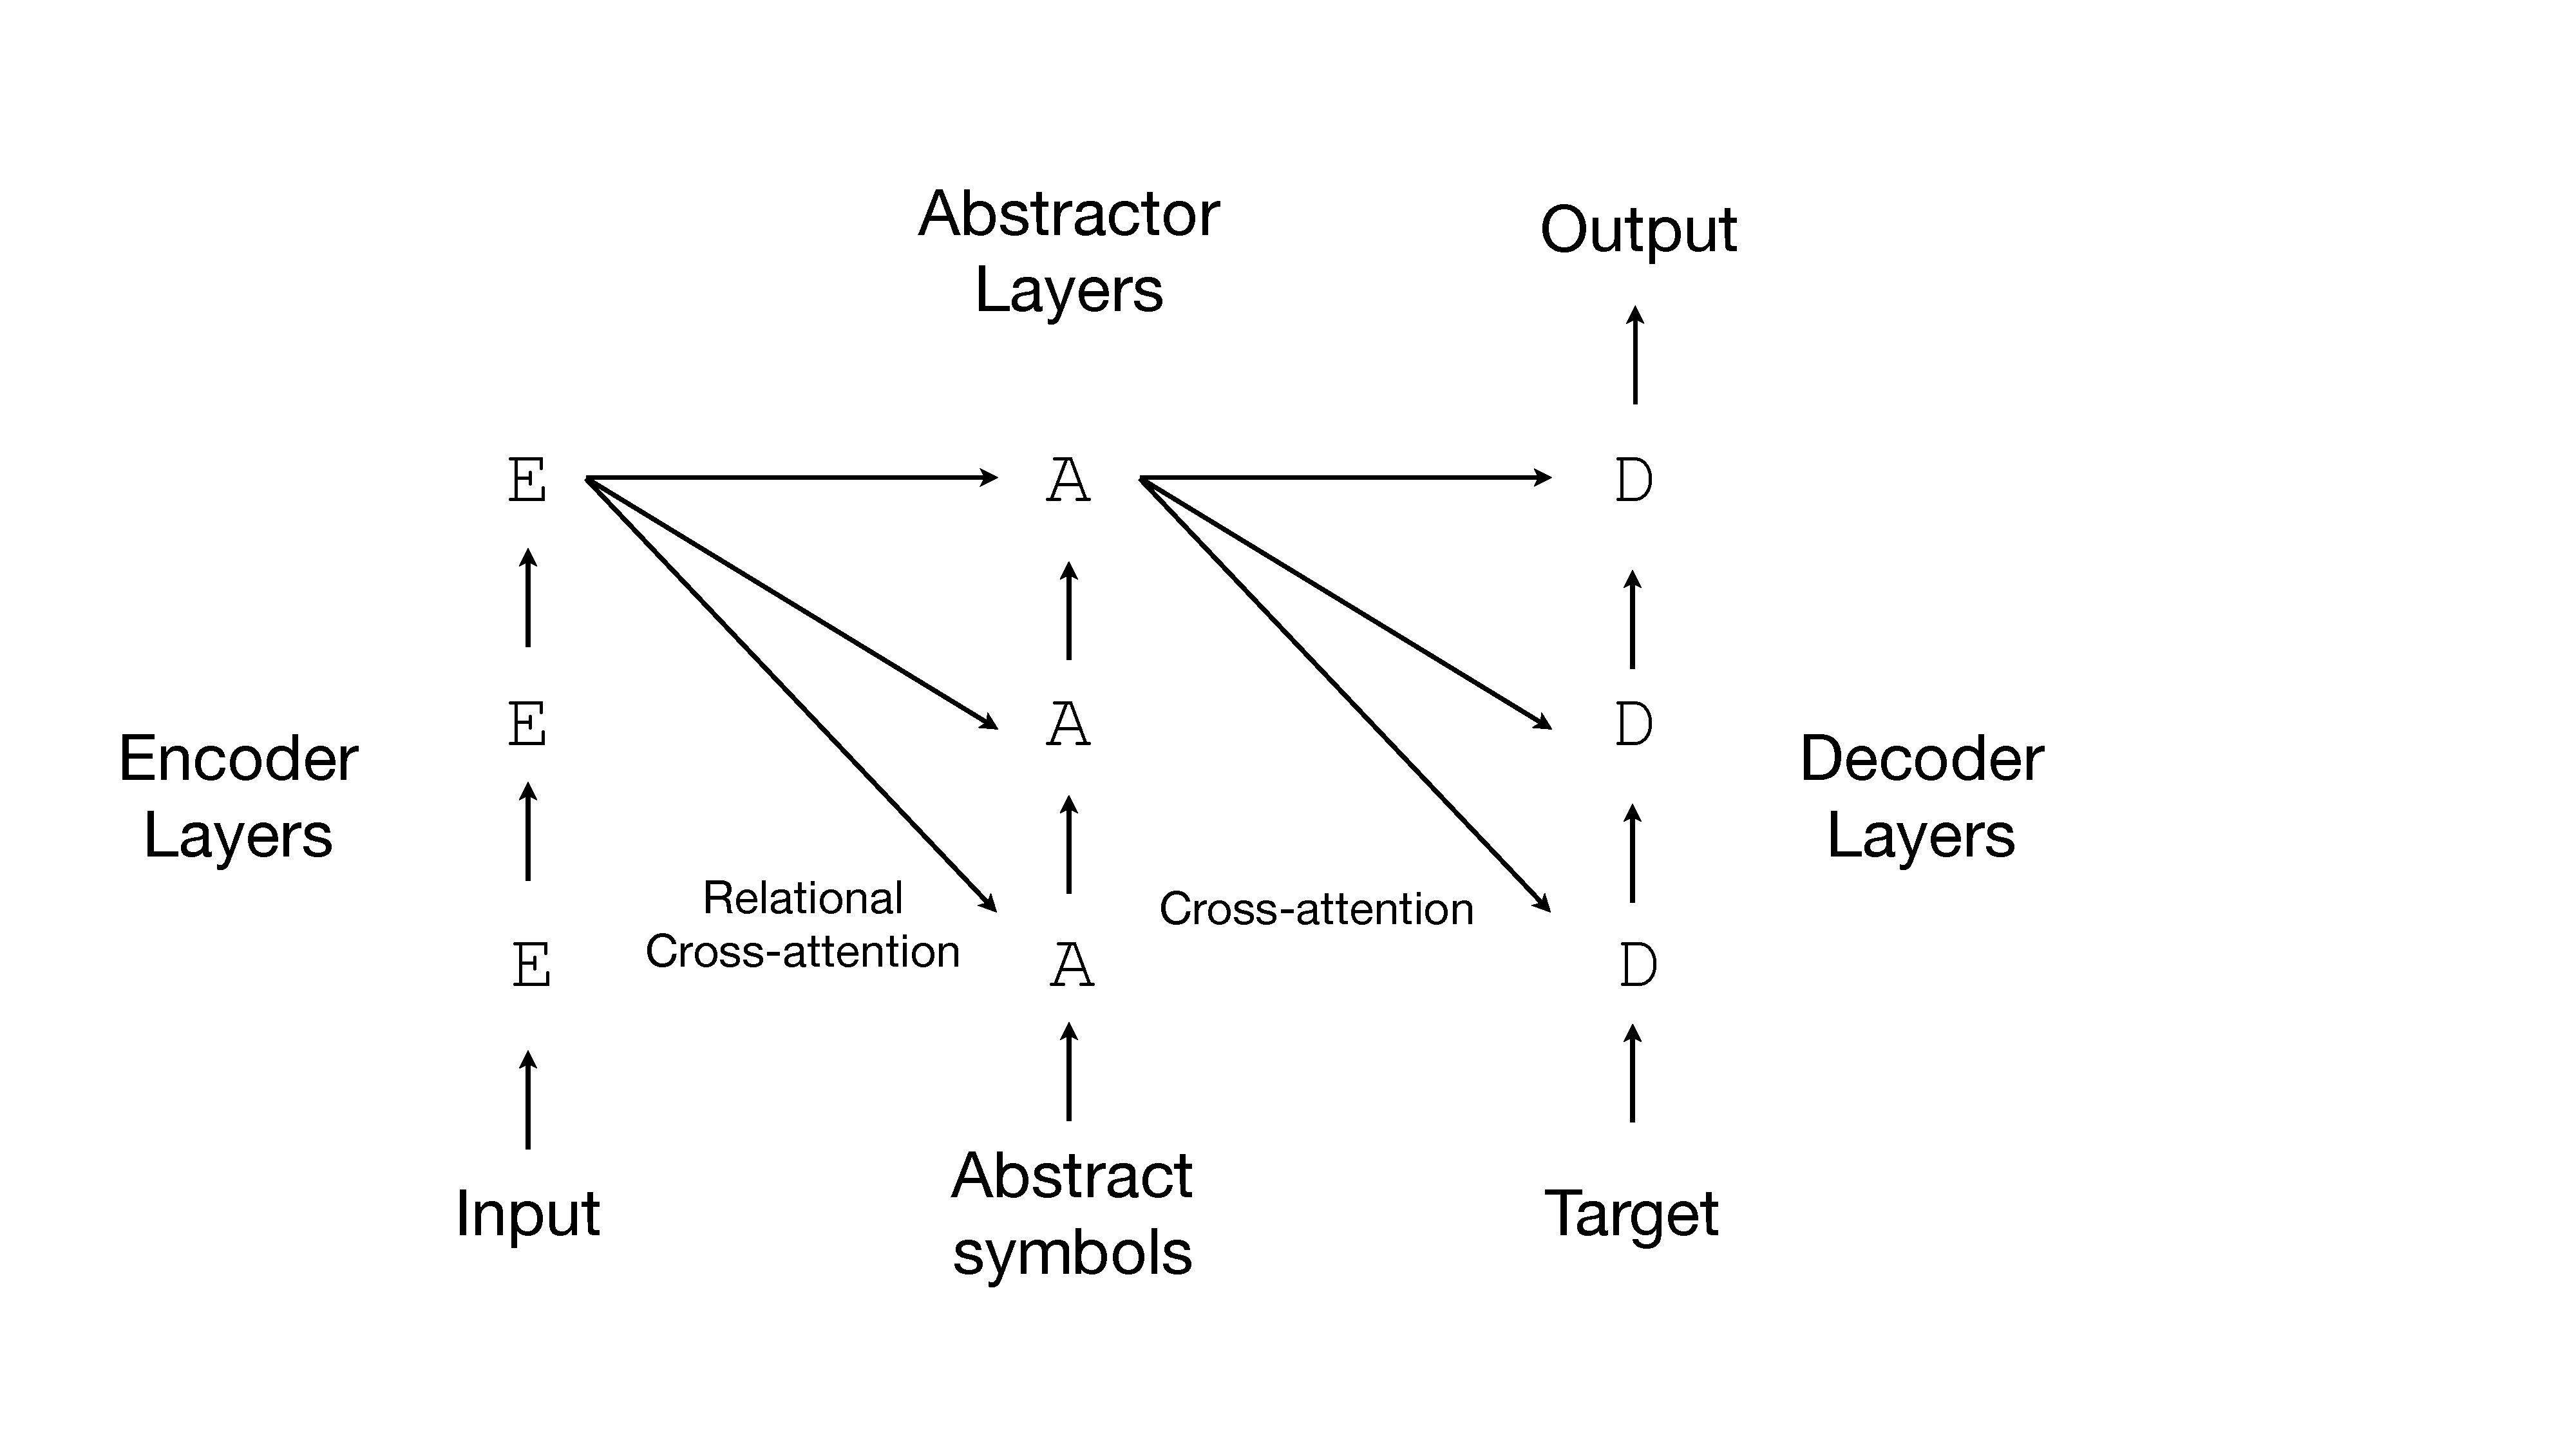
\includegraphics[width=.55\textwidth]{figures/algorithm-diagram3} 
    \end{tabular}
    \caption{Algorithmic framework integrating transformers and relational learning, with encoder/decoder layers for sensory/motor processes, and abstractor layers for representing relations between encoder and decoder states. Left: In general, the relational cross attention mechanisms can be regulated by a controller, and bindings between encoder/decoder and abstractor states are maintained in episodic memory. The architecture is motivated by principles of brain organization separating sensory processing from abstract reasoning and decision making. Right: Simplification in terms of a transformer architecture, where the abstract symbols depend only on relations between encoder states. %This allows abstract states---e.g., emergent symbols---to be shared and reused across problems and %domains, leading to data efficiency and generalization. When Encoder/Decoder states appear together %repeatedly through experience and replay, the abstract inference circuit can be preempted by a direct %connection (gray arrow), leading to computational efficiency and parallelization (i.e., consolidation %and automatization). 
    }
    \label{fig:algo}
    \vskip-12pt
    \end{center}
\end{figure}

\subsection{Relational cross-attention}


In transformers, attention is used to access convex combinations of vectors called \text{values}. The weights are normalized inner products between other vectors called the keys and queries, after mapping each with a separate, learned linear transformation. If the queries are the columns of a matrix $Q = (q_1,\ldots, q_m)\in\reals^{d_1\times m}$, the keys are the columns of a matrix $K = (k_1, \ldots, k_m)\in\reals^{d_1\times m}$, and the values are the columns a matrix $V\in\reals^{d_2\times m}$, then the cross-attention mechanism computes the convex combination in the column space of $V = (v_1, \ldots, v_m)$ given by 
\begin{align*}
    & V R  \\
    & R \equiv \softmax{K^T Q}
\end{align*}
with  the $\softmax{\cdot}$ operation applied column-wise. The $m\times m$ matrix $R = (r_{ij})$ is thought of 
as a relation between keys and values, computed in terms of inner products, with column $r_j$ 
encoding the relations between query $q_j$ and the keys $k_1, k_2, \ldots, k_m$. Thus, the transformed 
values are 
\begin{equation*}
    v_j \leftarrow V r_j = \sum_{i=1}^m r_{ij} v_i .
\end{equation*}

In standard transformers, the cross-attention mechanism between encoder states $E$ and decoder states $D$
uses queries $Q = AD$, keys $K = BE$, and values $V = CE$, where the matrices $A,B,C \in\reals^{d\times d}$ are 
linear transformations learned for each attention head.  We denote this with the notation 
\begin{equation*}
     \qkv{D}{E}{E}
\end{equation*}
where the linear transformations $A, B, C$ are not shown. The self-attention for the encoder 
states is then
\begin{equation*}
    \qkv{E}{E}{E}
\end{equation*}

Given the context of the encoder states $E$, a sequence of abstractor layers transforms the abstract symbols $A = (a_1,\ldots, a_m)$, using two types of attention: Self-attention $\qkv{A}{A}{A}$ and 
\textit{relational cross-attention} 
\begin{equation*}
    \qkv{E}{E}{A}.
\end{equation*} 
The initial abstract state is $S = (s_1,\ldots, s_m)$ 
with abstract symbols $s_j$ that are task-dependent but input-indendent, trainable using 
backpropagation. The relational cross-attention mechanism learns relations among the encoder states and use those relations to transform the abstract state. Importantly, the relational cross-attention heads 
encode learned relations and attributes, and can be reused across tasks.


Only relational information in the encoder states, computed through inner products, 
is used to transform the abstract variables; no information about the encoder states $E$ is directly accessed by the abstract side. For example, an attention head may learn to be directed toward the relevant dimension of an $E$ state (e.g., the color or shape of an object), without being associated with any particular value along that dimension. If the specific representation of $E$ changes, the same abstract relations will hold as long as the transformed inner products are approximately preserved. 



\subsection{Example}

We use the game SET to illustrate relational cross-attention. SET is a relatively straightforward but challenging cognitive task that engages reasoning faculties in a deliberative, attentionally directed manner, requiring several levels of abstraction over sensory embeddings. Players are presented with 12 cards, each of which contains figures that vary along four dimensions (color, number, pattern, and shape; see Figure \ref{fig_set}a) and they must find subsets of three cards which obey a simple but challenging rule: along each dimension, all cards in a set must either have the same or unique values (e.g., in Figure \ref{fig_set}, cards with two solid blue/purple diamonds, two striped blue squiggles, and two open blue oblongs: same color, same number, different patterns, different shapes). 

Algorithmically, task performance can be described as follows. The visual arrangement of cards is processed into a set of encoder states $E$ by standard deep learning mechanisms. The abstractor, starting in some initial abstract state $A$, transforms the state by the evaluation of attention heads that extract relations between the cards, each head giving a relation between them in a learned attribute. 

\def\redcard{\colorbox{red!30}{R}\hskip.2em}
\def\bluecard{\colorbox{blue!30}{B}\hskip.2em}
\def\greencard{\colorbox{green!50}{G}\hskip.2em}
\def\onecard{\fbox{\hskip1pt 1\hskip1pt}\hskip.2em}
\def\twocard{\fbox{\hskip1pt 2\hskip1pt}\hskip.2em}
\def\threecard{\fbox{\hskip1pt 3\hskip1pt}\hskip.2em}

\begin{figure}[t]
\begin{center}
\begin{tabular}{ccc}
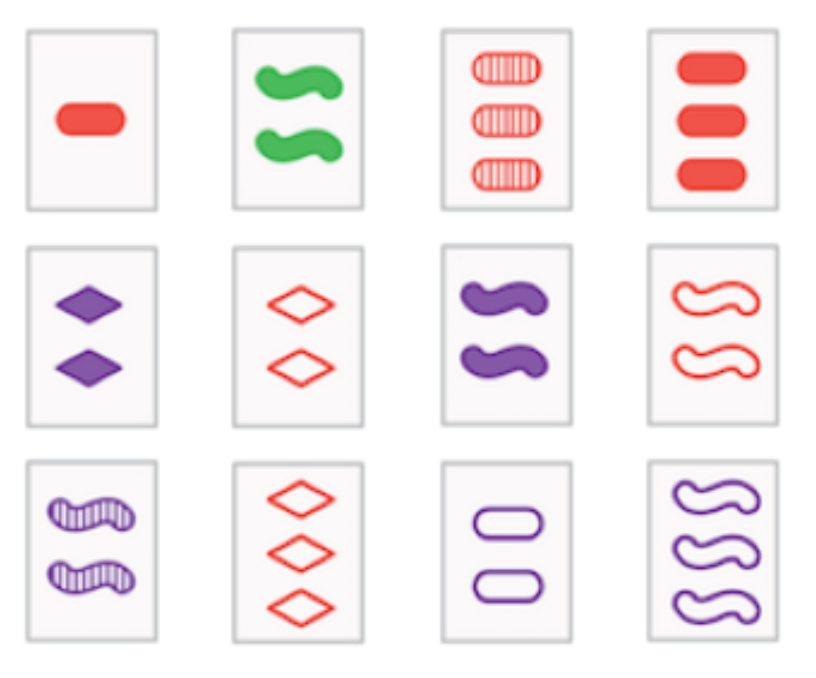
\includegraphics[width=.23\textwidth]{figures/set_example}
& &\\[-1.45in]
&\renewcommand{\arraystretch}{1.4}
\begin{small}
\begin{tabular}{|c|c|c|}
%\hline
\multicolumn{3}{c}{Attributes of encoder state $E=E_{1:3}$} \\
\hline
\multicolumn{1}{|c}{\redcard \redcard \redcard} & \multicolumn{1}{|c}{ \redcard\bluecard\greencard} &\multicolumn{1}{|c|}{\redcard\redcard\bluecard} \\
\hline
\hline
$\frac{1}{3}(A_1+A_2+A_3)$ & $\frac{1}{2}(A_2+A_3)$ & $A_3$ \\
$\frac{1}{3}(A_1+A_2+A_3)$ & $\frac{1}{2}(A_1+A_3)$ & $A_3$ \\
$\frac{1}{3}(A_1+A_2+A_3)$ & $\frac{1}{2}(A_1+A_2)$ & $\frac{1}{2}(A_1+A_2)$ \\
\hline
\multicolumn{3}{c}{Transformed abstract symbol $A=A_{1:3}$}
%\hline
\end{tabular}
\end{small}
%& \\[-1.45in]
%&&\includegraphics[width=.23\textwidth]{ppo-results/epoch_14_decision_boundaries} \vspace{-2mm} \\ 
\\[10pt]
\scriptsize (a) SET game & \scriptsize (b) Example of symbols/attention 
\end{tabular}
\vspace{-1mm}
\end{center}
\caption{Illustration of mechanism used in abstractor layers with relational cross attention using the game of SET (see text for description). 
%To provide a basic working of example of abstraction in our framework, 
As an example, consider an initial abstract symbol $A = A_{1:3}$ for three cards, and the color attribute.
%, for concreteness. 
Suppose a relation is learned such that  $\braket{E_i}{E_j}$ is large if cards $i$ and $j$ have different color, and is small if they are the same color.  Then relational cross-attention transforms the initial abstract symbol $A$ as shown in the above table. A multilayer perceptron can learn to discriminate between these three cases. Once learned, the symbol $A$ then can be used to represent abstract ``same/different'' relations for sequence of inputs.}
\label{fig_set}
\end{figure}


\begin{comment}
\def\redcard{\colorbox{red!30}{R}\hskip.1em}
\def\bluecard{\colorbox{blue!30}{B}\hskip.1em}
\def\greencard{\colorbox{green!50}{G}\hskip.1em}
\def\onecard{\fbox{\hskip2pt 1\hskip2pt}\hskip.1em}
\def\twocard{\fbox{\hskip2pt 2\hskip2pt}\hskip.1em}
\def\threecard{\fbox{\hskip2pt 3\hskip2pt}\hskip.1em}

\begin{figure}[htb]
\vspace{-2mm}
    \centering
    \begin{minipage}{0.46\linewidth}
        \centering
     %  \begin{table}[h]
\scriptsize
\centering
\begin{tabulary}{\columnwidth}{@{}p{0.1\columnwidth}p{0.25\columnwidth}p{0.25\columnwidth}p{0.2\columnwidth}@{}}
\toprule
Symbol  & \multicolumn{3}{c}{{Symbol mapped by relational cross attention $\braket{E}{E}\ket{A}$}}  \\
\cmidrule(r){1-1}     \cmidrule(lr){2-4}
%\toprule
$A_1$ & $(A_1+A_2+A_3)/3$ & $(A_2+A_3)/2$ & $A_3$ \\
\midrule
$A_2$ & $(A_1+A_2+A_3)/3$ & $(A_1+A_3)/2$ & $A_3$ \\
\midrule

$A_3$ & $(A_1+A_2+A_3)/3$ & $(A_1+A_2)/2$ & $(A_1+A_2)/2$ \\
 \bottomrule
Attributes $\bra{E}$: & \redcard \redcard \redcard & \redcard\bluecard\greencard & \redcard\redcard\bluecard \\
& \onecard \onecard \onecard & \onecard\twocard\threecard & \onecard\onecard\twocard
\end{tabulary}
%\end{table}
        \caption{Illustration of mechanism used in abstractor layers with relational cross attention using the game of SET (see text for description). 
%To provide a basic working of example of abstraction in our framework, 
As an example, consider an initial abstract symbol $A = A_{1:3}$ for three cards, and the color attribute.
%, for concreteness. 
Suppose a relation is learned such that  $\braket{E_i}{E_j}$ is large if cards $i$ and $j$ have different color, and is small if they are the same color.  Then relational cross-attention (approximately) transforms the initial abstract symbol $A$ as shown in the above table. A simple multilayer perceptron can learn to discriminate between these three cases with very little training data. Once learned, the symbol $A$ then can be used to represent abstract ``same/different'' relations for any triple of inputs, regardless of their sensory encoding.}
        \label{fig:perf-node}
    \end{minipage}%
        \hspace{3mm}%
  \begin{minipage}{.5\linewidth}
    \centering
    \includegraphics[width=\linewidth]{figures/pp_parallel.pdf}
    \caption {Parallelized execution of the \textit{Predator Prey XL} model.}
    \label{fig:perf-parallel}
 \end{minipage}%
\end{figure}
\end{comment}

\subsection{Configuring abstractors for different tasks}
\def\module#1{{\small\texttt{#1}}}

Abstractors can be used to approach a variety of relational learning tasks. In the case of classification 
or regression, the default architecture would be 
$$\module{Encoder} \rightarrow \module{Abstractor}$$
where the discriminant or regression function is computed as $f(A)$ where $A$ is the final abstract state.

For relational sequence-to-sequence tasks, the default architecture is 
$$\module{Encoder} \rightarrow \module{Abstractor} \rightarrow \module{Decoder}$$
In a ``fully relational'' task, the decoder can only attend to the abstractor, and therefore 
only uses relational information from the input. An example is sorting objects; we give 
experimental details for this example in Section~\ref{sec:experiments}.
In a ``partially-relational'' task, the decoder will attend to both the abstractor and encoder modules. In such cases, relational information is important to solving the task, but information about input ``values'' is 
also important. This provides an extension of general sequence-to-sequence models with transformers.


We note that composing abstractor modules, as in the architecture
$$\module{Encoder} \rightarrow \module{Abstractor} \rightarrow \module{Abstractor} \rightarrow \module{Decoder}$$
enables learning of higher order relations. To explain why, 


\def\rdot{\bigcdot}
\def\F{{\mathfrak{F}}}
\def\MLP{\text{MLP}}

\section{Function classes}
\label{sec:function_spaces}

In this section, we will discuss the class of relational functions computable by the symbolic message-passing operation in relational abstractors. We also comment on the robustness of these operations. In the process, we characterize the class of relational functions realizable by inner product relational neural networks, which may be of independent interest.

We start by presenting a universal approximation result for inner product relations. This will be useful when characterizing the class of functions computable by abstractors, but is also of interest more generally for relational machine learning.

\subsection{Function class of inner product relations}

A natural way to model relations between objects is through inner products between their vector representations. Consider vectors living in a space \(\mathcal{X}\). We would like to learn a relation function \(R: \mathcal{X} \times \mathcal{X} \to \reals^{d_r}\) which maps pairs of objects in \(\mathcal{X}\) to a \(d_r\)-dimensional vector describing the relation between these objects. We will model this relation function as a vector of inner products between transformations of the objects' representations:
\begin{equation}
	\label{eq:inner_product_relations}
	R(x, y) = \begin{pmatrix}\langle \phi_{1}(x), \phi_{1}(y) \rangle \\ \vdots \\ \langle \phi_{d_r}(x), \phi_{d_r}(y) \rangle \end{pmatrix},
\end{equation}
where \(\phi_{1}, \ldots, \phi_{d_r}\) are learnable transformations corresponding to each dimension of the relation. These transformations can be thought of as \textit{relational filters}. They extract a particular attribute of the objects such that an inner product of the transformed objects indicates the alignment or similarity along this attribute. Having several different filters allows for modeling rich multi-dimensional relations. This is one notable advantage of this formulation over the CoRelNet model \citep{kerg2022neural}, which processes a relation matrix as input to a multi-layer perceptron.

In a deep learning model, a natural choice is for \(\phi_{1}, \ldots, \phi_{d_r}\) to be \(d_r\) different neural networks (e.g.: MLPs, CNNs, etc. depending on the object space \(\mathcal{X}\)). Hence, the parameters of \(R\) are \(\boldsymbol{\theta} = (\theta_{1}, \ldots, \theta_{d_r})\), where \(\theta_{i}\) are the parameters of \(\phi_{i}\).

The following result characterizes the class of inner product relations computable by \eqref{eq:inner_product_relations} when \(\phi_{1}, \ldots, \phi_{d_r}\) are feedforward networks. We make use of Mercer's theorem and universal approximation properties of feedforward networks to obtain a universal approximation result for inner product relational neural networks.


\begin{thm}[Function class of inner product relational neural networks]
	\label{thm:function_class_inner_product_relnn}
	\hphantom{~}

	Consider an inner product relational neural network modeling a \(d_r\)-dimensional relation via inner products of neural networks,
	\begin{equation*}
		\langle x, y \rangle_{\MLP} := \begin{bmatrix}\langle \MLP_{\theta_1}(x), \MLP_{\theta_1}(y) \rangle \\ \vdots \\ \langle \MLP_{\theta_{d_r}}(x), \MLP_{\theta_{d_r}}(y) \rangle\end{bmatrix}.
	\end{equation*}

	Suppose the data lies in a compact Hausdorff space \(\mathcal{X}\) (e.g.: a metric space) with a finite countably additive measure. In particular, \(\mathcal{X}\) can be any compact subset of \(\mathbb{R}^d\).

	Then, \(\langle \cdot, \cdot \rangle_{\MLP}\) is a Mercer kernel along each of the \(d_r\) dimensions.

	Furthermore, for any vector-valued relation function \(R: \mathcal{X} \times \mathcal{X} \to \reals^{d_r}\) which is a Mercer kernel in each dimension, there exists an inner product relational neural network which approximates $R$ arbitrarily closely in the superemum norm (i.e.: uniformly over \((x,y) \in \mathcal{X}\times\mathcal{X}\)). More precisely, for all \(\epsilon > 0\), there exists \(d_r\) neural networks with parameters \(\theta_1, \ldots, \theta_{d_r}\) such that \(\sup_{x,y \in \mathcal{X}}{\lVert R(x,y) - \langle x, y \rangle_\MLP \rVert_\infty} < \epsilon\).
\end{thm}

\begin{proof}
	\hphantom{~}

	Denote the given relation function \(R\) by its \(d_r\) components:
	\begin{equation}
		R(x,y) = (R_1(x,y), \ldots, R_{d_r}(x,y)).
	\end{equation}
	By assumption, \(R_i\) is a Mercer kernel for each \(i = 1, \ldots, d_r\). Consider the component \(R_i\). By Mercer's theorem \citep{mercerFunctionsPositive1909, sunMercerTheorem2005, universal}, there exists \((\psi_i)_{i \in \mathbb{N}}\), \(\lambda_i \geq 0\) such that \(R_i(x,y) = \sum_{i=1}^{\infty}{\lambda_i \psi_i(x) \psi_i(y)}\), where \(\psi_i\) and \(\lambda_i\) are eigenfunctions and eigenvalues of the integral operator

	\begin{align*}
		T_R&: L_2(\mathcal{X}) \to L_2(\mathcal{X}) \\
		T_R(f) &= \int_{\mathcal{X}}{R(\cdot, x) f(x) dx}.
	\end{align*}

	Furthermore, the convergence of the series is uniform:
	\begin{equation}
		\lim_{n \to \infty} \sup_{x,y \in \mathcal{X}} \lvert R_i(x,y) - \sum_{j=1}^{n}{\lambda_j \psi_j(x) \psi_j(y) \rvert} = 0
	\end{equation}

	Let \(\tilde{n}_i\) be such that
	\begin{equation}
		\label{eq:proof_mercer_thm_unif_abs_cv}
		\sup_{x,y \in \mathcal{X}} \left\lvert R_i(x,y) - \sum_{j=1}^{n}{\lambda_j \psi_j(x) \psi_j(y)} \right\rvert < \frac{\epsilon}{2}
	\end{equation}

	Now, for \(j = 1, \ldots, \tilde{n}_i\), let the \(i\)th neural network with parameters \(\theta_i\) be a function from \(\mathcal{X}\) to \(\tilde{n}_i\)-dimensional space. Let \((\sqrt{\lambda_1} \psi_1, \ldots, \sqrt{\lambda_{\tilde{n}_i}} \psi_{\tilde{n}_i})\) be the function to be approximated by the \(i\)th neural network. By the universal approximation property of neural networks, for any \(\epsilon_1\), there exists a neural network with parameters \(\hat{\theta}_i\) such that
	\begin{equation}
		\label{eq:proof_NN_UAP}
		\sup_{x\in \mathcal{X}}{\left\lvert (\MLP(x))_j - \sqrt{\lambda_j} \psi_j(x) \right\lvert } < \epsilon_1
	\end{equation}

	We refer to \citep{hornikMultilayerFeedforward1989, cybenkoApproximationSuperpositions1989, barronUniversalApproximation1993} for results guaranteeing the existence of neural networks which can approximate any continuous function over a bounded domain.

	For ease of notation, we denote \(\MLP_{\hat{\theta}_i}\) simply by \(\MLP\), omitting the dependence on fixed \(i\). Furthermore, \(\MLP(x)_j\) is the \(j\)th component of the output of \(\MLP(x)\). Now note that the approximation error for \(R_i\) is bounded by
	\begin{equation}
		\label{eq:proof_approx_bound}
		\begin{split}
			\sup_{x, y \in \mathcal{X}}&{
				\left\lvert R_i(x,y) - \langle \MLP(x), \MLP(y) \rangle \right\rvert}\\
			&= \sup_{x, y \in \mathcal{X}}{
				\left\lvert R_i(x,y) - \sum_{j=1}^{\tilde{n}_i}{\MLP(x)_j \MLP(y)_j} \right\rvert} \\
			&\leq \sup_{x,y \in \mathcal{X}}{ \left(
				\left\lvert R_i(x,y) - \sum_{j=1}^{\tilde{n}_i}{\lambda_j \psi_j(x) \psi_j(y)} \right\rvert
				+ \left\lvert \sum_{j=1}^{\tilde{n}_i}{\lambda_i \psi_j(x) \psi_i(y) - \MLP(x)_j \MLP(y)_j} \right\rvert  \right) }
		\end{split}
	\end{equation}
	The first term is less than \(\frac{\epsilon}{2}\) by \eqref{eq:proof_mercer_thm_unif_abs_cv}. The second term can be bounded uniformly on \(x,y\) by
	\begin{equation*}
		\begin{split}
			&\left\lvert \left(\sum_{j=1}^{\tilde{n}_i}{\lambda_i \psi_j(x) \psi_i(y)}\right) - \langle \MLP(x), \MLP(y) \rangle \right\rvert  \\
			&\leq \sum_{j=1}^{\tilde{n}_i}{ \left\lvert \lambda_i \psi_j(x) \psi_i(y) - \MLP(x)_j \MLP(y)_j \right\rvert} \\
			&\leq \sum_{j=1}^{\tilde{n}_i}{\left(
				\left\lvert \MLP(x)_j \right\rvert \left\lvert \sqrt{\lambda_j} \psi_j(y) - \MLP(y)_j \right\rvert
				+ \lvert \MLP(y)_j \rvert \left\lvert \sqrt{\lambda_j} \psi_j(x) - \MLP(x)_j \right\rvert
				\right)}
		\end{split}
	\end{equation*}
	Let \(\epsilon_1\) in \eqref{eq:proof_NN_UAP} be small enough such that the above is smaller than \(\frac{\epsilon}{2}\). 	Then, by \eqref{eq:proof_approx_bound}, we have that
	\begin{equation*}
		\sup_{x, y \in \mathcal{X}}{
			\lvert R_i(x,y) - \langle \MLP(x), \MLP(y) \rangle \rvert} \leq \frac{\epsilon}{2} + \frac{\epsilon}{2} = \epsilon
	\end{equation*}

	We repeat this for each component of the relation function \(R_i\), \(i=1, \ldots, d_r\), obtaining \(d_r\) neural networks each with parameters \(\hat{\theta}_i\). Thus, \(\sup_{x,y \in \mathcal{X}}{\lVert R(x,y) - \langle x, y \rangle_\MLP \rVert_\infty} < \epsilon\).
\end{proof}

\begin{remark}
	The result also holds for universal approximators other than feedforward neural networks, with a nearly identical proof.
\end{remark}

\Cref{thm:function_class_inner_product_relnn} shows that an inner product relational neural network can approximate arbitrary continuous, symmetric, positive semi-definite relation functions \(R(\cdot, \cdot)\). We now make a couple of remarks.

Learning the relation function in equation \eqref{eq:inner_product_relations} involves learning \(d_r\) different non-linear transformations \(\phi_{1}, \ldots, \phi_{d_r}\). To enable greater weight-sharing, we can instead have a single non-linear learned function \(\phi: \mathcal{X} \to \mathbb{R}^{\tilde{d}}\) along with \(d_r\) linear projections \(W_k \in \mathbb{R}^{m \times \tilde{d}}\), such that
\begin{equation}
	\label{eq:weight_sharing_inner_product_relnn}
	R(x,y) = \begin{pmatrix}\langle W_1 \phi(x), W_1 \phi(y) \rangle \\ \vdots \\ \langle W_{d_r}\phi(x), W_{d_r}\phi(y) \rangle\end{pmatrix}.
\end{equation}
This is does not shrink the class of computable relation functions since for any set of learned functions \(\phi_1, \ldots, \phi_{d_r}\) in the former set up, we can consider a single \(\phi\) which is simply a concatenation of all these outputs and have the linear projections extract the appropriate components.

Additionally, we can consider inner products of the form
\begin{equation}
	\label{eq:nonsymmetric_inner_product_relnn}
	\langle W_k^{(1)} \phi(x_i), W_k^{(2)} \phi(x_j) \rangle,
\end{equation}
\noindent where the linear projections for the first and second entities may be different, in order to achieve non-symmetric relation functions. This yields a strictly larger class of relation functions than in Theorem \ref{thm:function_class_inner_product_relnn}.

This is closely related to the cross-attention operation in transformers (and  abstractors). In cross-attention, the relation between two objects is given by an inner product between the two object vectors transformed by a `query' matrix and a `key' matrix respectively: \(\langle W_Q x, W_K y \rangle\). A `relation tensor' giving pairwise relations is then computed as \(\Softmax((W_K X)^\top (W_Q X))\), where \(X = \begin{bmatrix} x_1 & \cdots & x_\m\end{bmatrix}\) are the object vectors. The multiple heads of multi-head attention similarly correspond to the multi-dimensional relations modeled by the transformations \(\phi_{1}, \ldots, \phi_{d_r}\) in the inner product relational neural network \ref{eq:inner_product_relations}.

\begin{remark}
	The function class of non-symmetric inner product relational neural networks of the form
	\[ R(x,y) = \begin{pmatrix}
		\langle \phi_1(x), \psi_1(y) \\
		\vdots \\
		\langle \phi_{d_r}(x), \psi_{d_r}(y)
	\end{pmatrix}\]
	can also be characterized.
\end{remark}

\subsection{Class of relational functions computable by symbolic message-passing}
\label{ssec:function_class_symbolic_mp}
For the purposes of this analysis, the algorithmic description of symbolic message-passing is presented in \Cref{alg:symbolic_mp}. It is slightly simpler than the algorithmic description of the full relational  abstractor in \Cref{alg:relational_abstractor}---the primary difference is that we omit self-attention between symbolic states.

\begin{algorithm}[ht!]
	\caption{Symbolic Message-Passing}\label{alg:symbolic_mp}
	\SetKwInOut{Input}{Input}
	\SetKwInOut{Output}{Output}
	\SetKwInOut{LearnableParams}{Learnable parameters{\ }}
	\SetKwInOut{HyperParams}{Hyperparameters}

	\Input{Relation tensor: \(R \in \mathbb{R}^{n \times \m \times d_r}\)}
	\HyperParams{\(L\) (number of steps/layers), hyperparameters of feedforward networks}
	\LearnableParams{symbols \(\boldsymbol{s} = (s_1, \ldots, s_\m) \in \reals^{d_s \times \m}\), feedforward neural networks \(\phi^{(1)}, \ldots, \phi^{(L)}\)}
	\Output{Abstracted sequence: \(\boldsymbol{a} = (a_1, \ldots, a _\m) \in \reals^{d_a \times \m}\)}
	\vspace{1em}

	\(A \gets S\)

	\For{\(l \gets 1\) \KwTo \(L\)}{
		\(a_i \gets \sum_{j=1}^{n} R[i,j] a_j, \quad i = 1, \ldots, n\)

		\(a_i \gets \phi^{(l)}(a_i), \quad i = 1, \ldots, n\)
	}
\end{algorithm}



From equation \eqref{eq:linear_symbolic_mp}, the symbolic message-passing operation is clearly bijective as a function on the input relation tensor \(R\), for an appropriate choice of the symbol parameters \(S = (s_1,\ldots, s_\m)\). For example, choosing \(S = I_{\m \times \m}\) (i.e.: the \(i\)th symbolic vector is the indicator \(\m\)-vector with a \(1\) in the \(i\)th position, \(s_i = e_i\)) reproduces the relation tensor after one message-passing operation:
\begin{equation*}
	s_i  \leftarrow  \sum_{j=1}^{n} R[i,j] e_j = \begin{pmatrix}R[i,1] \\ R[i,2] \\ \vdots \\ R[i,n]\end{pmatrix}.
\end{equation*}
More generally, one linear step of symbolic message-passing yields updated symbolic vectors such that \(s_i'\) is a linear function of the vector of all objects' relations with object \(i\):
\begin{equation*}
	s_i \leftarrow = S \begin{pmatrix}R[i,1] \\ \vdots \\ R[i,n]\end{pmatrix}.
\end{equation*}
Following the linear step in symbolic message-passing, each updated symbolic state is transformed via a neural network. Hence, the \(i\)th abstracted value after symbolic message-passing is given by
\begin{equation*}
	a_i = \phi\left(S r_i \right),
\end{equation*}
where \(\phi\) is a neural network, and \(R_i\) is the vector of object \(i\)'s relations with every other object, \(R_i = \begin{pmatrix}R[i,1] & \cdots & R[i,n]\end{pmatrix}^\top\). Hence, \(a_i\) summarizes all the information about object \(i\)'s relations to all other objects. We summarize this discussion by the following
lemma, which follows from universal approximation properties of feed-forward networks.

\begin{lemma}
	\label{lemma:function_class_1_step_symbolic_mp}
	A one-step symbolic message-passing operation (in \Cref{alg:symbolic_mp}) can compute arbitrary functions of a each object's relations with other objects in the input sequence. That is, there exists a choice of symbols \(s_1, \ldots, s _\m\) and parameters of the feed-forward network such that \(a_i\) computes an arbitrary function of object \(i\)'s relations, \(r_i = \begin{pmatrix}R[i,1] & R[i,2] & \cdots & R[i,n]\end{pmatrix}^\top\).
\end{lemma}


Thus, the abstracted sequence after a single step of symbolic message-passing has the form
\begin{equation}
	\label{eq:abstracted_seq_1_layer_abstractor}
	A^{(1)} = (a_1^{(1)}, \ldots, a_\m^{(1)}) = \left(\phi(r_1), \phi(r_2), \ldots, \phi(r_\m)\right),
\end{equation}
where \(\phi\) is an arbitrary learnable function shared by all abstracted objects, and \(r_i\) is the vector of object \(i\)'s relations with every other object.

That is, \(a_i^{(1)}\) summarizes object \(i\)'s relations with other objects. With further symbolic message-passing operations, the \(i\)th abstracted vector can be made to represent information about other relations, not necessarily involving the \(i\)th object. For example, at the second layer, the abstracted vectors take the form
\begin{equation}
	a_i^{(2)} = \phi^{(2)} \left( \sum_{j=1}^{n} R[i,j] a_j^{(1)} \right) = \phi^{(2)} \left( \sum_{j=1}^{n} R[i,j] \phi^{(1)}(R_j) \right).
\end{equation}

We conclude this subsection by remarking that the above analysis concerns \Cref{alg:symbolic_mp}---a simplified version of the relational  abstractor. In particular, while it captures the effects of relational cross-attention, it does not include self-attention on the abstract symbols. The analysis indicates that we should expect the function class generated by a relational  abstractor module in \Cref{alg:relational_abstractor} to be no smaller than that of the simple symbolic message-passing in \Cref{alg:symbolic_mp}.


\subsection{Composing  abstractors to compute relations on relations}
\label{ssec:compsing_abstractors}

As described in \Cref{sec:abstractors_as_transformer_modules}, the abstactor framework supports composing  abstractors in the form
\begin{equation*}
	\texttt{Encoder} \to \texttt{Abstractor} \to \cdots \to \texttt{Abstractor} \to \texttt{Output}
\end{equation*}
Here, we analyze the function class generated by a composition of several abstractors. We make the simplifying assumption that each single layer abstractor takes the simplified form of the symbolic message-passing operation in \Cref{alg:symbolic_mp}. This corresponds to omitting the self-attention operation in \Cref{alg:relational_abstractor} while maintaining the relational cross-attention with the sequence of output vectors at the previous  abstractor.

We saw in the previous section that a one-layer abstractor is able to compute arbitrary functions  of each object's relations. Observe that the output sequence of abstracted objects is a sequence of `relational vectors'. That is, objects which summarize relational information. Hence, chaining together a sequence of  abstractors allows the computation of relations on relations.

% TODO: formalize or refine presentation of result
\begin{lemma}
	\label{lemma:function_class_composed_abstractors}
	A chain of \(k\) single-layer  abstractors is able to compute arbitrary ``\(k\)th order relational functions'' in the sense of the proof below.
\end{lemma}
\begin{proof}[Proof sketch]
	In \Cref{ssec:function_class_symbolic_mp} we characterized the output of a 1-layer abstractor as
	\begin{equation*}
		A^{(1)} = (a_1^{(1)}, \ldots, a_\m^{(1)}) = \left(\phi^{(1)}(r_1), \phi^{(1)}(r_2), \ldots, \phi^{(1)}(r_\m)\right),
	\end{equation*}
	Note that we will now use the superscript to denote the abstractor in the chain rather than the layer depth in a single  abstractor, as all  abstractors have a depth of one.

	Let the second abstractor's symbols be denoted by \(S^{(2)} = (s_1^{(2)}, \ldots, s_\m^{(2)})\). Then,
	\begin{equation*}
		a_i^{(2)} = S^{(2)} \begin{bmatrix}R^{(2)}[i,1] \\ \vdots \\ R^{(2)}[i,n]\end{bmatrix},
	\end{equation*}
	where,
	\begin{equation*}
		R^{(2)} = \Softmax\left((W_K A^{(1)})^\top (W_Q A^{(1)})\right).
	\end{equation*}
	Observe that
	\begin{equation*}
		\left[(W_K A^{(1)})^\top (W_Q A^{(1)})\right]_{ij} = \langle W_Q \phi^{(1)}(r_j), W_K \phi^{(1)}(r_i) \rangle.
	\end{equation*}
	By Theorem \ref{thm:function_class_inner_product_relnn}, composing an arbitrary learnable function \(\phi\) with inner products enables learning arbitrary relation functions on the input space (i.e.: any continuous, symmetric, positive semi-definite bivariate function. Here, the class of functions is actually larger since it allows for non-symmetric relation functions when \(W_Q \neq W_K\)).

	In the above, the space over which we are computing relations is itself a space of relation vectors. That is, \(\langle W_Q \phi^{(1)}(R_j), W_K \phi^{(1)}(R_i) \rangle\) computes a relation between object \(i\)'s relations and object \(j\)'s relations. Hence, choosing \(s_i^{(2)} = e_i\) and ignoring the Softmax for now, yields
	\begin{equation*}
		a_i^{(2)} = \phi^{(2)}\left(\begin{bmatrix}\langle W_Q \phi^{(1)}(r_i), W_K \phi^{(1)}(r_1) \rangle \\ \vdots \\ \langle W_Q \phi^{(1)}(r_i), W_K \phi^{(1)}(r_\m) \rangle\end{bmatrix}\right).
	\end{equation*}
	Thus, \(a_i^{(2)}\) computes arbitrary second-order relation functions. Namely, it computes arbitrary relations between object \(i\)'s relation vector and every other object's relation vector.

	More generally, at layer \(l\), we have
	\begin{align*}
		R^{(l)} &= \Softmax\left((W_K A^{(l-1)})^\top (W_Q A^{(l-1)})\right),\\
		a_i^{(l)} &= \phi^{(l)}\left(S^{(l)} \begin{bmatrix}R^{(l)}[i,1] \\ \vdots \\ R^{(l)}[i,n]\end{bmatrix}\right).
	\end{align*}
	Thus, \(R^{(l)}\) computes \(l\)th order-relations, and \(a_i^{(l)}\) is a linear map applied to the \(l\)th-order relations involving object \(i\).
\end{proof}


\subsection{Robustness and error correction}

For the relational cross-attention mechanism used by abstrators, an \(m\times m\) relation
is computed as  \(R = \mbox{Softmax}(K^T Q)\)
and relational cross attention then transforms the symbols by
\(A = SR\) so that each abstract variable \(a_j\) is in the convex hull of the set of symbols.
As long as \(S\) has rank \(m\), relations are uniquely determined from the abstract symbols.
Here we point out how the transformed symbols can be robust to noise if the symbols are
sufficiently redundant.

Specifically, suppose that the symbols \(S\) are transformed to \(A\) and corrupted with additive noise:
\begin{equation}
  A = SR + \Xi
\end{equation}
where a fraction \(\epsilon\) of the entries of \(\Xi\) are drawn from an adversarial noise distribution, and the other entries are zero; dropout noise is also possible.
This can be studied as an instance of compressed sensing and ``model repair'' \citep{candes_randall,model_repair}.  In particular, the relations can be recovered using the  robust regression estimator
\begin{equation}
  \hat r_j = \argmin_{u \in\reals^m} \| a_j - S u\|_1 \label{eq:lp}
\end{equation}
where \(A = (a_1,a_2,\ldots, a_m)\) with columns \(a_j\in\reals^d\).
The main lemma in \cite{model_repair} states that the following two conditions suffice:

\underline{Condition A:}
  There exists some \(\sigma^2\), such that for any fixed \(c_1,...,c_d\) satisfying \(\max_i|c_i|\leq 1\),
  \begin{equation}
    \left\|\frac{1}{d}\sum_{i=1}^d c_i s_{i\rdot} \right\|^2\leq \frac{\sigma^2 m}{d},
  \end{equation}
with high probability, where \(s_{i\rdot}\in\reals^m\) is the \(i\)th row of \(S\).

\underline{Condition B:}
  There exist \(\underline{\kappa}\) and \(\overline{\kappa}\), such that
  \begin{eqnarray}
  \label{eq:l1-upper-A} \inf_{\|\Delta\|=1}\frac{1}{d}\sum_{i=1}^d|s_{i\rdot}^T\Delta| &\geq& \underline{\kappa}, \\
  \label{eq:l2-upper-A} \sup_{\|\Delta\|=1}\frac{1}{d}\sum_{i=1}^d|s_{i\rdot}^T\Delta|^2 &\leq& \overline{\kappa}^2,
  \end{eqnarray}
  with high probability.

\begin{thm}\label{thm:main-improved}
  Assume the symbol matrix \(S\) satisfies Condition A and Condition B. Then if
  \begin{equation}
  \frac{\overline{\kappa}\sqrt{\frac{m}{d}\log\left(\frac{e d}{k}\right)}+\epsilon\sigma\sqrt{\frac{m}{d}}}{\underline{\kappa}(1-\epsilon)}
  \end{equation}
  is sufficiently small, the linear program \eqref{eq:lp} recovers \(R\), so that \(\hat r_j = r_j\) with high probability.
  \end{thm}

The condition is essentially that
  \begin{equation}
    \frac{1}{1-\epsilon} \sqrt{\frac{m}{d}}
  \end{equation}
  is small, meaning that the dimension \(d\) of the symbols needs to be sufficiently large relative
  to the dimension \(k\) of the relation.

  \subsection{Sparse, high-dimensional relations}

 The above setting ensures enough redundancy to recover the relations, constraining the number of symbols \(k\) to be small relative to the symbol dimension \(d\). This is not appropriate in the situation where the relations are over a large number \(m\) of elements, for example, the contents of the entire episodic memory.
 In this setting we assume that the relation tensor \(R \in \reals^{m\times m}\) is sparse; that is,
 each column \(r_j \in \Delta_m\) has at most \(k\) nonzero entries: \(\|r_j\|_0 \leq k\). To recover the relation
 we now use the robust lasso estimator, which is a related linear program
\begin{equation}
  \hat r_j = \argmin_{u \in\reals^m} \| a_j - S u\|_1 + \lambda\|u\|_1. \label{eq:rlasso}
\end{equation}
Here we have an analogous theorem, stating that if
\begin{eqnarray}
  \frac{\overline{\kappa}/\underline{\kappa}}{1-\epsilon}\sqrt{\frac{k}{d}\log(2m)}\leq c,
\end{eqnarray}
for some sufficiently small constant \(c>0\), the robust lasso estimator \eqref{eq:rlasso} satisfies
\begin{equation}
  \|\hat r_j - r_j\| \leq C \frac{\overline{\kappa}/\underline{\kappa}^2}{1-\epsilon} \sqrt{\frac{\sigma^2 k}{d} \log(2m)}
\end{equation}
for some constant \(C\).
This implies that we can accurately recover the relation tensor in the high dimensional setting, even when many of the entries of the transformed abstract symbols are corrupted.


The above discussion shows how the relation tensor can be recovered from the transformed symbols, even under adversarial noise, assuming there is sufficient redundancy in the symbols. This implies that it is possible to predict as well from the transformed symbols as from the relations, without explicitly recovering the relations.
Using ideas from \citep{surfing,HandV17}, it may be possible to extend this theory to nonlinear mappings
\(y = \varphi(Au) + \eta\) where \(\varphi(\cdot)\) is an activation function.
%; this could serve as an alternative to the Hopfield model of memory retrieval and pattern completion.



\section{Experiments}\label{sec:experiments}

\footnotetext{\footnotesize We ran the experiments described here on RTX 2080ti, RTX 3090, and A100 GPUs, available to us through our institution's internal cluster. The models here are relatively small; powerful GPUs are not required to train a single model. We found the use of GPUs useful for evaluating learning curves over several trials.}

\subsection{Warm up: Ability to learn asymmetric and multi-dimensional relations}
One recent work on relational machine learning is~\cite{kerg2022neural} where, based on prior work~\cite{esbn}, the
authors argue for a particular type of inductive bias in relational models and propose CorelNet. The architecture is: given a sequence of objects $(x_1, \ldots, x_m)$, embed them using an MLP $\phi$, then compute the similarity matrix $R = \text{Softmax}(A), A = {\left[\langle\phi(x_i), \phi(x_j)\rangle\right]}_{ij}$. The final output is an MLP applied to the flattened similarity matrix. They demonstrate that this model can solve a series of simple tasks with high sample-efficiency compared to models like ESBN and standard Transformers. However, CorelNet has some notable limitations. One is that, as described,
it is only able to model symmetric relations\footnote{This is not fundamental to the CoRelNet model, which can learn asymmetric relations via the natural modification $A = {\left[\langle W_1 \phi(x_i), W_2 \phi(x_j)\rangle\right]}_{ij}$, where $W_1, W_2$ are trainable matrices.}---$R$ is symmetric by definition.
Another limitation is that it can only model single-dimensional relations---for each pair of objects $(i,j)$, their modeled relation is a single-dimensional scalar $R_{ij}$. The Abstractor is able to model a significantly larger class of relations. In particular, it is able to model asymmetric and multi-dimensional relations through the $\text{MultiHeadRelation}$ operation. This is demonstrated by the following simple experiment. Note that this is merely intended as a warm up; we don't wish to imply that this task is not solvable by standard models which lack a relational bottleneck (see the following experiments for more interesting comparisons).

We generate $N = 32$ ``random objects'' represented by iid Gaussian vectors, $o_i \overset{iid}{\sim} \mathcal{N}(0,
I_d) \in \mathbb{R}^d$, and associate an order relation to them $o_1 \prec o_2 \prec \cdots \prec o_N$. We train
several different relational models to learn this order relation. Note that $\prec$ is \textit{not symmetric}. Of the $N^2 = 1024$ possible pairs $(o_i, o_j)$, 15\% are held out as a validation set (for early stopping) and 35\% as a test set. We evaluate learning curves by training on the remaining 50\% and computing accuracy on the test set (10 trials for each training set size). Note that under this set up, we are evaluating the models on pairs they have never seen. Thus, the models will need to generalize based on the transitivity of the $\prec$ relation. We observe that a simple Abstractor model is able to learn the relation while CorelNet cannot~(\Cref{fig:exp_order_relation}).

For completeness, we also compare to a standard Transformer model. The transformer model performs slightly better than the Abstractor on this simple task. We include this to highlight that an Abstractor will not necessarily be superior to a Transformer uniformly on all tasks, but rather that it can realize significant gains on tasks with complex relational structure (see the following experiments).

\begin{figure*}
    \vskip-.2in
    \begin{subfigure}[t]{0.40\textwidth}
        %\centering
        \hskip-.35in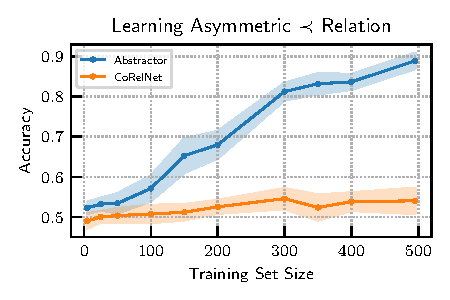
\includegraphics[scale=.95]{figures/experiments/pairwise_order_learning_curves.pdf}
        \vskip-5pt
        \caption{The Abstractor learns the transitive $\prec$ relation and generalizes, whereas CorelNet's learning curve is flat at the baseline accuracy of 0.5.}\label{fig:exp_order_relation}
    \end{subfigure} \hspace{\fill}
    \captionsetup[subfigure]{oneside,margin={-.3in,0in}}
    \begin{subfigure}[t]{0.40\textwidth}
        %\centering
        % \vskip10pt
        \hskip-.6in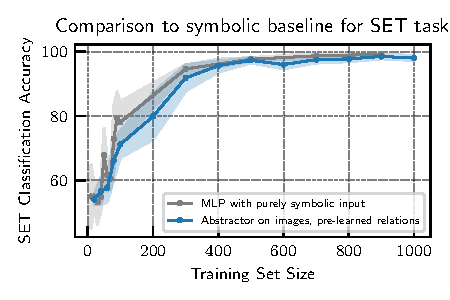
\includegraphics[scale=.95]{figures/experiments/set_symbolic_vs_abstractor.pdf}
        \vskip-5pt
        \caption{Comparison of Abstractor trained on images of cards and MLP with relations hand-encoded symbolically as bit vectors.}% The Abstractor is nearly as sample efficient as symbolic computation.}
        \label{fig:exp_set}
    \end{subfigure}

    \begin{subfigure}[t]{0.40\textwidth}
        %\centering
        \hskip-.35in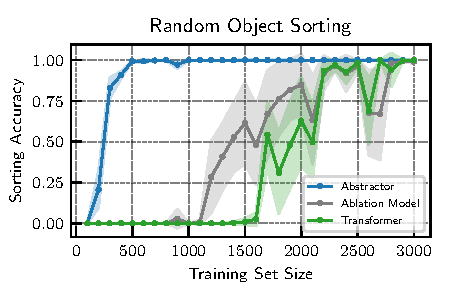
\includegraphics[scale=.95]{figures/experiments/random_object_sorting.pdf}
        \vskip-5pt
        \caption{Learning curves on sorting sequences of random objects. The abstractor is dramatically more sample-efficient.}\label{fig:exp_object_sorting}
    \end{subfigure}\hspace{\fill}
    \begin{subfigure}[t]{0.40\textwidth}
        %\centering
        \hskip-.6in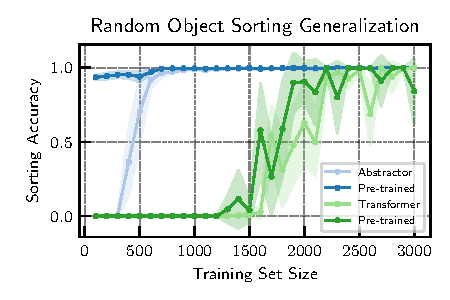
\includegraphics[scale=.95]{figures/experiments/random_object_sorting_generalization.pdf}
        \vskip-5pt
        \caption{Learning curves with and without pre-training on a similar sorting task. The Abstractor benefits significantly from pre-training.}\label{fig:exp_object_sorting_generalization}
    \end{subfigure}
    % \bigskip

    \begin{subfigure}[t]{0.40\textwidth}
        %\centering
        \hskip-.35in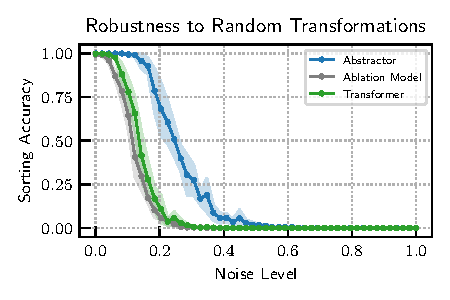
\includegraphics[scale=.95]{figures/experiments/additive_robustness.pdf}
        \vskip-5pt
        \caption{The Abstractor is more robust to corruption by additive noise. }\label{fig:exp_robustness}
    \end{subfigure}\hspace{\fill}
    \begin{subfigure}[t]{0.40\textwidth}
        %\centering
        \hskip-.6in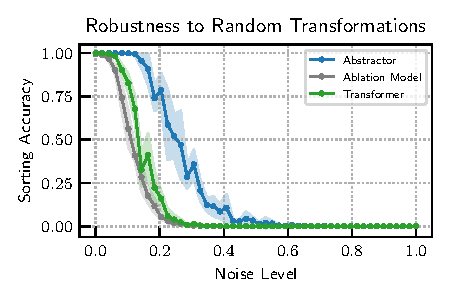
\includegraphics[scale=.95]{figures/experiments/multiplicative_robustness.pdf}
        \vskip-5pt
        \caption{The Abstractor is more robust to corruption by a random linear transformation.}\label{fig:exp_robustness2}
    \end{subfigure}

    \caption{Experiments. Shaded regions indicate twice the standard error of mean.}\label{fig:experiments}
    \vskip-.10in
\end{figure*}

\subsection{Superior sample-efficiency on relational tasks compared to plain transformers}
The next experiment extends the idea of learning an order relation $\prec$ on random objects: now, the task is to fully sort sequences of randomly permuted random objects.

We generate random objects in the following way. First, we generate two sets of random attributes $\mathcal{A} = \{a_1, a_2, a_3, a_4\}$, $a_i \overset{iid}{\sim} \mathcal{N}(0, I) \in \mathbb{R}^{4}$ and $\mathcal{B} = \{b_1, \ldots, b_{12}\}$, $b_i \overset{iid}{\sim} \mathcal{N}(0, I) \in \mathbb{R}^{8}$. To each set of attributes, we associate the strict ordering relation $a_1 \prec a_2 \prec a_3 \prec a_4$ and $b_1 \prec b_2 \prec \cdots \prec b_{12}$, respectively. Our random objects are formed by the Cartesian product of these two attributes $\mathcal{O} = \mathcal{A} \times \mathcal{B}$, yielding $N = 4 \times 12 = 48$ objects (i.e., each object in $\mathcal{O}$ is a vector in $\mathbb{R}^{4+8}$ formed by a concatenation of one attribute value in $\mathcal{A}$ and one in $\mathcal{B}$). Then, we associate with $\mathcal{O}$ the strict ordering relation corresponding to the order relation of $\mathcal{A}$ as the primary key and the order relation of $\mathcal{B}$ as the secondary key. i.e., $(a_i, b_j) \prec (a_k, b_l)$ if $a_i \prec a_k$ or if $a_i = a_k$ and $b_j \prec b_l$.

Given a set of objects in $\mathcal{O}$, the task is to sort it according to $\prec$. More precisely, the input sequences are randomly permuted sequences of $10$ objects in $\mathcal{O}$ and the target sequences are the indices of the object sequences in sorted order (i.e., the `argsort'). The training data are sampled uniformly from the set of length-10 sequences in $\mathcal{O}$. We also generate a non-overlapping validation dataset (used during training for early stopping) and a testing dataset (used during evaluation).

We evaluate learning curves on an Abstractor, a Transformer, and an ``Ablation'' model (10 trials for each training set size). The Abstractor uses the architecture $\texttt{Encoder} \to \texttt{Abstractor} \to \texttt{Decoder}$. The Encoder-to-Abstractor interface uses relational cross-attention and the Abstractor-to-Decoder interface uses standard cross-attention. The Ablation Model aims to test the effects of the relational cross-attention in the Abstractor model---it is architecturally identical to the Abstractor model with the crucial exception that the Encoder-to-Abstractor interface instead uses standard cross-attention. The hyperparameters of the models are chosen so that the parameter counts are similar. % TODO: add details here? or in supplement?
We find that the Abstractor is dramatically more sample-efficient than the Transformer and the Ablation model~(\Cref{fig:exp_object_sorting}).

\subsection{Ability to generalize to similar tasks}

Continuing with the object-sorting task and the dataset generated as described above, we test the Abstractor's ability to generalize from similar relational tasks through pre-training. The main task uses the same dataset described above. The pre-training task involves the same object set $\mathcal{O}$ but the order relation is changed. The ordering in attribute $\mathcal{A}$ is randomly permuted, while the ordering in attribute $\mathcal{B}$ is kept the same. A strict ordering relation $\prec$ on $\mathcal{O}$ is obtained in the same way---using the order in $\mathcal{A}$ as the primary key and the order in $\mathcal{B}$ as the secondary key.

The Abstractor model here uses the architecture $\texttt{Abstractor} \to \texttt{Decoder}$ (i.e., no Transformer
encoder), and the transformer is the same as the previous section. We pre-train both models on the pre-training task
and then, using those learned weights for initialization, evaluate learning curves on the original task. Since the
Transformer requires more training samples to learn the object-sorting task, we use a pre-training set size of $3,000$, chosen based on the results of the previous subsection so that it is large enough for the Transformer to learn the pre-training task. This experiment assesses the models' ability to generalize relations learned on one task to a new task.~\Cref{fig:exp_object_sorting_generalization} shows the learning curves for each model with and without pre-training. We observe that when the Abstractor is pre-trained, its learning curve on the object-sorting task is significantly accelerated. The transformer does not benefit from pre-training.

\subsection{Robustness and Out-of-Distribution generalization}
In this experiment, we evaluate robustness to a particular type of noisy corruption. We train each model on the same
object-sorting task described above. We use a fixed training set size of $3,000$ for the same reason
---it is large enough that all models are able to learn the task. On the hold out test set, we corrupt the object
representations by applying a random linear transformation. In particular, we randomly sample a random matrix the
entries of which are iid zero-mean Gaussian with variance $\sigma^2$, $\Phi \in \mathbb{R}^{d \times d}, \Phi_{ij} \sim \mathcal{N}(0, \sigma^2)$. Each object in $\mathcal{O}$ is then corrupted by this random linear transformation,
$\tilde{o}_i = \Phi o_i, \ \text{ for each } i \in [48]$. We also test robustness to additive noise via $\tilde{o}_i = o_i + \varepsilon_i, \varepsilon_i \sim \mathcal{N}(0, \sigma^2 I_d)$.

The models are evaluated on the hold-out test set with objects replaced by their corrupted version. We evaluate the sorting accuracy of each model while varying the noise level $\sigma$ (5 trials at each noise level). The results are shown in figures~\ref{fig:exp_robustness} and~\ref{fig:exp_robustness2}. We emphasize that the models are trained only on the original objects in $\mathcal{O}$, and are not trained on objects corrupted by any kind of noise.

This experiment can be interpreted in two lights: the first is robustness to noise. The second is a form of out-of
-distribution generalization. Note that the objects seen by the models post-corruption lie in a different space than
those seen during training. Hence the models need to learn relations that
are in some sense independent of the value representation.
As a theoretical justification for this behavior,~\cite{zhouCompressedPrivacySensitive2009} shows that $\langle \Phi x, \Phi y \rangle \approx \langle x, y \rangle$ in high dimensions, for a random matrix $\Phi$ with iid Gaussian entries. This indicates that models whose primary computations are performed via inner products, like Abstractors, may be more robust to this kind of corruption.

\subsection{Modularity and comparison to purely symbolic representations}
\label{ssec:set_exp}


\begin{wrapfigure}{R}{0.25\textwidth}
	\vskip-5pt
	\begin{tabular}{c}
		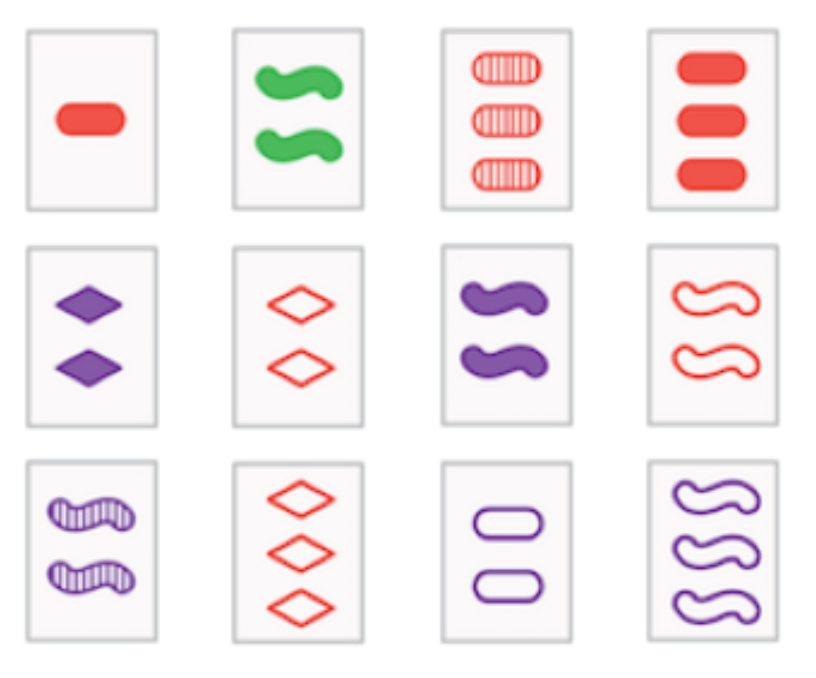
\includegraphics[width=.25\textwidth]{figures/set_example}\\[-5pt]
	\end{tabular}
	\caption{\footnotesize The SET game}
\end{wrapfigure}
SET is a relatively straightforward but challenging cognitive task that engages reasoning faculties in a deliberative
, attentionally directed manner, requiring several levels of abstraction over sensory embeddings. Players are
presented with 12 cards, each of which contains figures that vary along four dimensions (color, number, pattern, and
shape) and they must find subsets of three cards which obey a deceptively simple rule: along each dimension, all cards in a SET must either have the same or unique values.
% JDC: DO FIGURES NEED TO BE NUMBERED?
For example, in the figure to the right, the cards with two solid blue/purple diamonds, two striped blue squiggles, and two open blue oblongs form a SET: same color, same number, different patterns, different shapes.

To simulate the task of deciding if a triple forms a SET, we first train a convolutional neural network to process the color images of the cards (a full deck includes 81 cards). The CNN is trained to predict the attribute of
each card, as a multi-label classification, and then an embedding of dimension $d=32$ of 
each card is obtained. This embedding layer uses an \MLP{} to map the convolutional feature maps into a distributed
representation. Next, we train Abstractors separately for each of the four attributes to learn same/different
relations, where the task is to decide if an input pair of cards is the same or different for that attribute. 
We then use the query and key mappings $W_Q$ and $W_K$ learned for these relations to initialize the relations
in a multi-head Abstractor. The Abstractor is then trained on a dataset of triples of cards, half of which form a SET. 

This is compared to a baseline symbolic model where, instead of images, the input is a vector with 12 bits,
explicitly encoding the relations. That is, for each of the four attributes, a binary symbol is computed for each pair of three input cards---1 if the pair is the same in that attribute, and 0 otherwise. A two-layer MLP is then trained to decide if the triple forms a SET. The MLP using the symbolic representation can be considered as a lower bound on the performance achievable by the Abstractor. This comparison shows that the Abstractor is able to solve a task using relations learned in other tasks (modularity), with a sample efficiency that is not far from that obtained
with purely symbolic, noise-free encodings of the relevant relations. %We note that this uses a simple Abstractor configuration, without self-attention.

% JDC: I REALIZE WE ARE TIGHT ON SPACE, BUT IF THERE IS ROOM, COULD ADD THE FOLLOWING, OR A SHORTENED FORM OF
This subtask suggets how Abstractors might be viewed as an intermediate between strong ``nativist'' approaches that assume a pre-existing foundation of symbolic primitives and purely ``empiricist'' approaches that assume
similar capabilities can emerge simply from processing large amounts of data \cite{howtogrowamind}.
%can be achieved simply by the application of general purpose learning algorithms to large
%amounts of data -- showing how the latter, agumented with simple architectural inductive biases and trained using
%plausible and practical forms of curricular learninng both to generate genuinely symbolic representations, and use these to achieve the flexibilty and efficiency characteristic of human reasoning.
\footnote{We ran the experiments described here on RTX 2080ti, RTX 3090, and A100 GPUs which we had available to us via our institute's internal cluster. The models here are relatively small; powerful GPUs are not required to train a single model. We found the use of GPUs useful for evaluating learning curves over several trials.}

%\section{Introduction: The Relational Bottleneck}

\section{Relational Abstracters}

\noindent\textbf{Symbols} ...

\noindent\textbf{Relational Cross-Attention} ...

\noindent\textbf{Relational-Symbolic Message-Passing} ...

\section{Relational Abstracters as modules in a Transformer}
\subsection{Relational Classification Tasks}
$$\texttt{Encoder} \to \texttt{Abstracter}$$

\subsection{Sequence-to-Sequence Relational Tasks}
$$\texttt{Encoder} \to \texttt{Abstracter} \to \texttt{Decoder}$$

\noindent\textbf{Fully Relational Tasks}: decoder can attend only to abstracter. only needs relational information.

\noindent\textbf{Partially-Relational Tasks}: decoder attends to both abstracter and encoder. relational information is important to solving task, but `value' information and more general sequence-modeling is also relevant. Hence, attend to both encoder (as in standard transformer) and relational abstracter (as in above models). 

\subsection{Multi-Attention Decoders: Attending to both Encoder and Abstracter}

\subsection{Chaining Abstracters to Learn Higher-Order Relations}

\section{Characterizing the Function Class Generated by Relational-Symbolic Message-Passing}

\section{Experiments: Sorting Random-Objects}

\begin{itemize}
    \item sorting is a natural `relational' task: relations = ordering.
    \item consider a set of $N$ objects, $\{o_1, ..., o_N\}$ with associated ordering $o_1 \prec o_2 \prec \cdots \prec o_N$. objects are described by, for example, random vectors (or images, etc.). task: given a subset of the objects, sort it. requires understanding the relations between these objects.
    \item describe experimental set up and present results 
\end{itemize}

\section{Discussion}

\section*{Code and Data Availability}




\setlength{\bibsep}{8pt plus 0.3ex}
\bibliographystyle{apalike}
\bibliography{references}

\end{document}

\clearpage
\setcounter{section}{0}
\section{Introduction: The Relational Bottleneck}

\section{Relational Abstracters}

\noindent\textbf{Symbols} ...

\noindent\textbf{Relational Cross-Attention} ...

\noindent\textbf{Relational-Symbolic Message-Passing} ...

\section{Relational Abstracters as modules in a Transformer}
\subsection{Relational Classification Tasks}
$$\texttt{Encoder} \to \texttt{Abstracter}$$

\subsection{Sequence-to-Sequence Relational Tasks}
$$\texttt{Encoder} \to \texttt{Abstracter} \to \texttt{Decoder}$$

\noindent\textbf{Fully Relational Tasks}: decoder can attend only to abstracter. only needs relational information.

\noindent\textbf{Partially-Relational Tasks}: decoder attends to both abstracter and encoder. relational information is important to solving task, but `value' information and more general sequence-modeling is also relevant. Hence, attend to both encoder (as in standard transformer) and relational abstracter (as in above models). 

\subsection{Multi-Attention Decoders: Attending to both Encoder and Abstracter}

\subsection{Chaining Abstracters to Learn Higher-Order Relations}

\section{Characterizing the Function Class Generated by Relational-Symbolic Message-Passing}

\section{Experiments: Sorting Random-Objects}

\begin{itemize}
    \item sorting is a natural `relational' task: relations = ordering.
    \item consider a set of $N$ objects, $\{o_1, ..., o_N\}$ with associated ordering $o_1 \prec o_2 \prec \cdots \prec o_N$. objects are described by, for example, random vectors (or images, etc.). task: given a subset of the objects, sort it. requires understanding the relations between these objects.
    \item describe experimental set up and present results 
\end{itemize}

\section{Discussion}

\section*{Code and Data Availability}




\end{document}
